\chapter{Methodology}
The methodology for this dissertation is rigorously structured around the \textbf{Cross-Industry Standard Process for Data Mining (CRISP-DM)} framework. This framework on Figure~\ref{fig:crispdm} provides a systematic and iterative roadmap, ensuring that the technical development of the integrated Kiswahili speech analysis system remains aligned with practical application and stakeholder requirements, spanning from the initial understanding of the problem to final architectural deployment \citep{shearer2000crispdm,ibmcrispdm}.

\begin{figure}[H] % H forces the figure to appear exactly here (requires the float package)
    \centering
    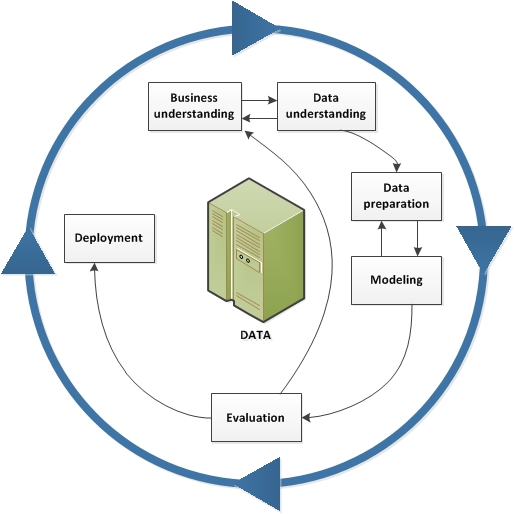
\includegraphics[width=0.8\textwidth]{images/crisp_process.jpg}
    \caption{The CRISP-DM Process Model (Adapted from IBM SPSS Modeler documentation).}
    \label{fig:crispdm}
\end{figure}

\section{Business Understanding}
The initial phase of the CRISP-DM framework is centered on defining the project objectives from a business perspective. This end-to-end pipeline is designed to benefit a diverse range of stakeholders who currently face significant challenges in processing spoken Kiswahili. Primary beneficiaries include customer service centers, which can use the system to automatically analyze customer feedback; media and content companies, which can efficiently transcribe and summarize broadcast content; and the education and governance sectors. In education, the system can be used to analyze classroom discourse to improve pedagogical strategies or develop automated tools for language learning \citep{shearer2000crispdm}. For governance, it provides a crucial tool for summarizing public feedback from community forums, tracking sentiment on policy changes, and gaining real-time insights from citizen feedback hotlines. By providing an automated, low-latency solution, this research will empower these organizations to transform unstructured spoken data into actionable intelligence, thus saving time and resources. Ultimately, this system serves as a foundational tool to democratize access to and analysis of information, directly promoting digital inclusion for the Kiswahili-speaking community.

The Business Understanding phase serves as the critical conceptual foundation of the project, identifying specific linguistic and technological "pain points" in the processing of Kiswahili digital data and translating them into tangible technical requirements.

\subsection{Background and Business Objectives}
Kiswahili stands as a cornerstone of communication for over 200 million individuals across East and Central Africa. Yet, within the global Artificial Intelligence ecosystem, it remains relegated to low-resource status. Historical development in Automatic Speech Recognition (ASR) and Natural Language Processing (NLP) has prioritized Indo-European languages like English and French, creating a digital divide that limits Kiswahili speakers' access to modern education and the digital economy. 

The central ambition of this research is to dismantle these barriers by engineering an end-to-end pipeline capable of converting raw Kiswahili audio into structured, actionable intelligence. By automating the extraction of insights from unstructured vocal data, this system aims to optimize resource allocation across four transformative sectors. In the realm of \textbf{customer experience}, the pipeline automates feedback analysis to identify service trends without manual intervention. For \textbf{media monitoring}, it enables the efficient indexing and archival of broadcast content for rapid searchability. Within \textbf{educational technology}, the system transcribes classroom discourse to produce automated learning aids and digital notes, while in \textbf{civic governance}, it provides a vital mechanism for summarizing citizen feedback and tracking real-time public sentiment.

\subsection{Assessment of the Situation}
A pragmatic deployment of this technology requires addressing several linguistic and operational hurdles. Kiswahili is characterized by intricate morphological structures and diverse regional dialects, often punctuated by Sheng or English code-switching \citep{Abdullah_Rusli_2021}. Beyond linguistics, the operational environment often involves limited computational power and intermittent connectivity in rural or low-income areas. To be viable, the pipeline must be engineered for high computational efficiency, ensuring it can perform on standard hardware with the minimal latency required for near real-time processing in media and service environments.

\subsection{Data Mining Goals}
To realize these objectives, the project is structured around four technical milestones. The first milestone focuses on \textbf{transcription accuracy} by fine-tuning Wav2Vec 2.0 architectures to achieve a minimal Word Error Rate (WER) specifically for the Swahili language. Second, we implement \textbf{sentiment extraction} using a DistilBERT-based classifier to categorize transcriptions into positive, negative, or neutral strata for rapid feedback analysis. Third, the project utilizes a Text-to-Text Transfer Transformer (T5) model for \textbf{summarization}, ensuring the core intent of long-form audio is preserved in a concise text format. Finally, \textbf{deployment viability} is achieved by integrating these models into a high-performance FastAPI prototype, demonstrating a seamless, low-latency transition from raw audio input to the final aggregated insights.

\subsection{Success Criteria}
Project success is measured by both technical and functional benchmarks. Technically, success is achieved if the pipeline demonstrates accuracy and reliability comparable to established baselines, validated through domain-specific metrics such as WER for transcription, F1-score for sentiment analysis, and ROUGE/BLEU scores for summarization. Functionally, success is defined by the successful integration of these distinct deep learning models into a cohesive, web-based interface that provides a seamless "one-stop" solution for Kiswahili speech analysis. Ultimately, the research aims to provide a foundational tool that fosters digital inclusion and information accessibility for the Kiswahili-speaking community.

\section{Data Understanding and Collection}
The Data Understanding phase represents a critical investigative stage within the CRISP-DM framework, involving the acquisition of the primary linguistic corpus and a multi-dimensional analysis of its technical and demographic characteristics. This stage ensures that the empirical foundation is sufficient to support the requirements of the multi-task pipeline.

\subsection{Data Acquisition and Source}
The research utilizes the Mozilla Common Voice Corpus 11.0 for Swahili (sw), a premier open-source dataset specifically engineered for the development of Automatic Speech Recognition (ASR) systems. This dataset is compiled through a massive crowdsourcing effort hosted by the Mozilla Foundation, where volunteers contribute recordings of themselves reading prompts. For the purposes of this study, the dataset comprises 14.76 GB of raw Swahili audio data, representing approximately 26,614 individual entries. A defining feature of this source is its built-in peer-validation mechanism; every clip designated as "validated" has successfully passed a review process where multiple contributors voted on the accuracy and clarity of the audio-to-text alignment.

\subsection{Data Description and Structural Schema}
A structural audit of the raw data was conducted to map the metadata schema and identify the features available for modeling. The corpus contains seven core columns that provide essential context for each recording. The speaker’s identity is managed via an anonymized unique identifier, while the file system path and the actual audio data stored as a numerical array with an associated sampling rate form the primary input for the ASR module. The target Swahili transcription is stored as a text object. Additionally, peer-validation metrics are tracked through integer counts of "up votes" and "down votes," which indicate the level of community agreement on clip quality. Demographic metadata, such as age and gender, is also present as object data, though these are voluntarily provided by the contributors.

\subsection{Exploratory Data Analysis and Quality Assessment}
Following the data collection phase, a comprehensive Exploratory Data Analysis (EDA) was performed to evaluate demographic representation and technical integrity. This audit revealed a significant concentration within the 20--29 age demographic, which accounts for approximately 52\% of the disclosed age data as shownas in Figure~\ref{fig:age_dist}.

\begin{figure}[h]
\centering
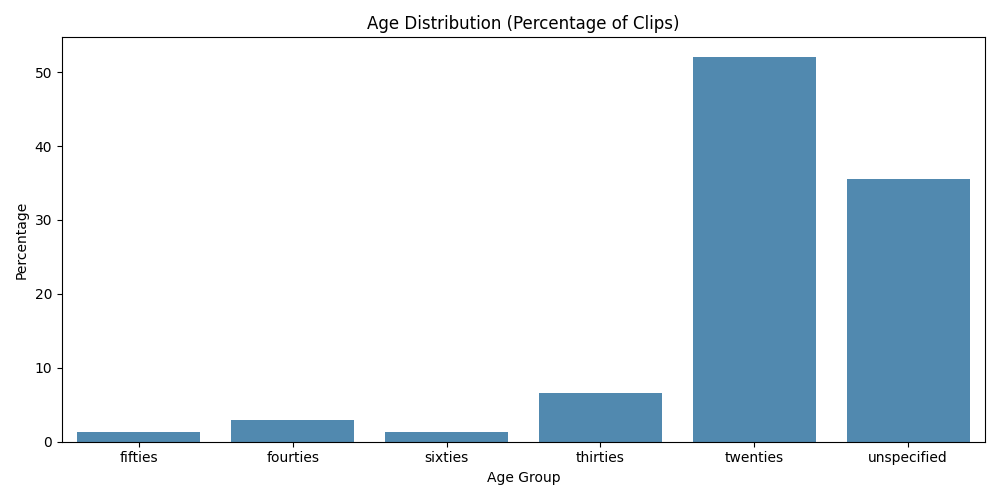
\includegraphics[width=0.8\textwidth]{images/age_distribution_cleaned.pdf}
\caption{Age distribution of contributors in the Swahili Common Voice corpus}
\label{fig:age_dist}
\end{figure}

In contrast, older age groups, specifically those over 50, are significantly underrepresented, comprising only 2.6\% of the corpus. The gender distribution similarly exhibits a skew, with female speakers representing 36.7\% and male speakers representing 27.7\%, while 35.6\% of the metadata remained undisclosed as revealed in Figure~\ref{fig:gender_dist}. 

\begin{figure}[h]
\centering
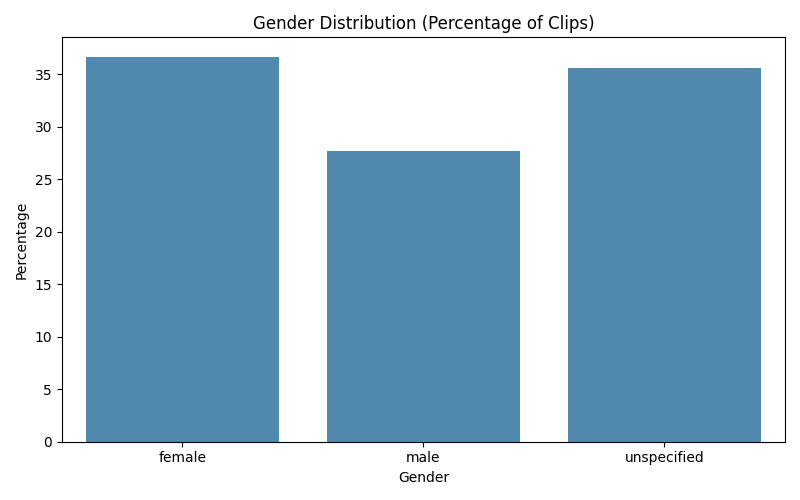
\includegraphics[width=0.8\textwidth]{images/gender_distribution_cleaned.pdf}
\caption{Gender distribution of contributors including undisclosed metadata}
\label{fig:gender_dist}
\end{figure}

To mitigate this missingness and maintain data integrity during model training, a neutral placeholder strategy was adopted to categorize unspecified entries.

\noindent The technical quality analysis was further informed by contributor and validation metrics. The dataset includes contributions from approximately 76 unique speakers. The calculated validation ratio, representing the proportion of down-votes to total votes, stands at 0.1287. This indicates that roughly 12.8\% of the data was flagged for potential quality issues by the community, providing a clear justification for the rigorous cleaning protocols implemented in the subsequent data preparation phase. A bivariate correlation analysis between transcript length and rejection rates (Pearson $r = 0.004$) revealed no meaningful relationship between the length of a sentence and the likelihood of it being down-voted, as illustrated in Figure~\ref{fig:vote_length}. 

\begin{figure}[h]
\centering
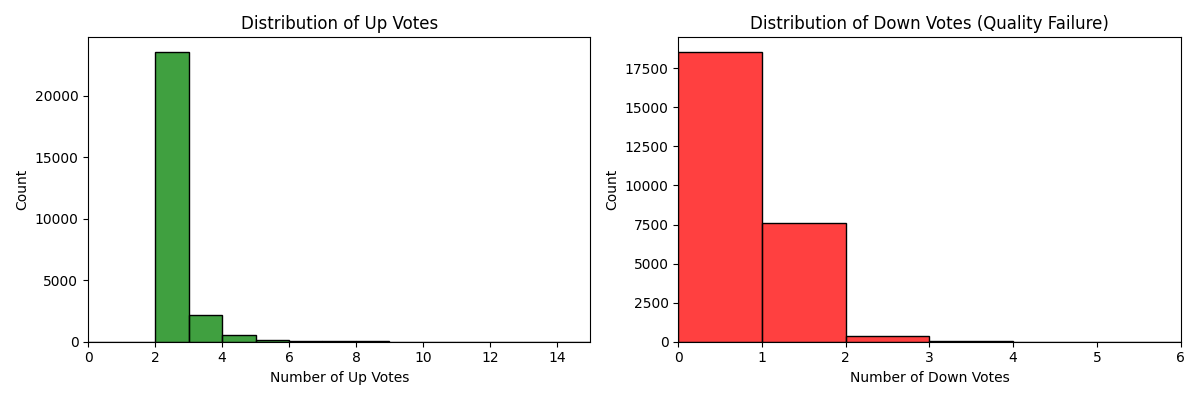
\includegraphics[width=0.85\textwidth]{images/votes_distribution.pdf}
\caption{Relationship between sentence length and down-vote ratio}
\label{fig:vote_length}
\end{figure}

This suggests that validation failures are primarily driven by acoustic factors, such as background noise or articulation, rather than the linguistic complexity of the prompts.

\noindent The linguistic characterization of the corpus revealed a median sentence length of 9.0 words and a mean word length of 5.46 characters. N-gram frequency analysis in Figure~\ref{fig:bigrams} highlighted the phrasal backbone of the dataset, with unigrams such as "ya", "na", and "wa" appearing with the highest frequency. Bigram analysis identified critical phrasal patterns such as "elfu moja", "baada ya", and "moja mia", which are essential for maintaining semantic coherence during transcription. 

\begin{figure}[H]
\centering
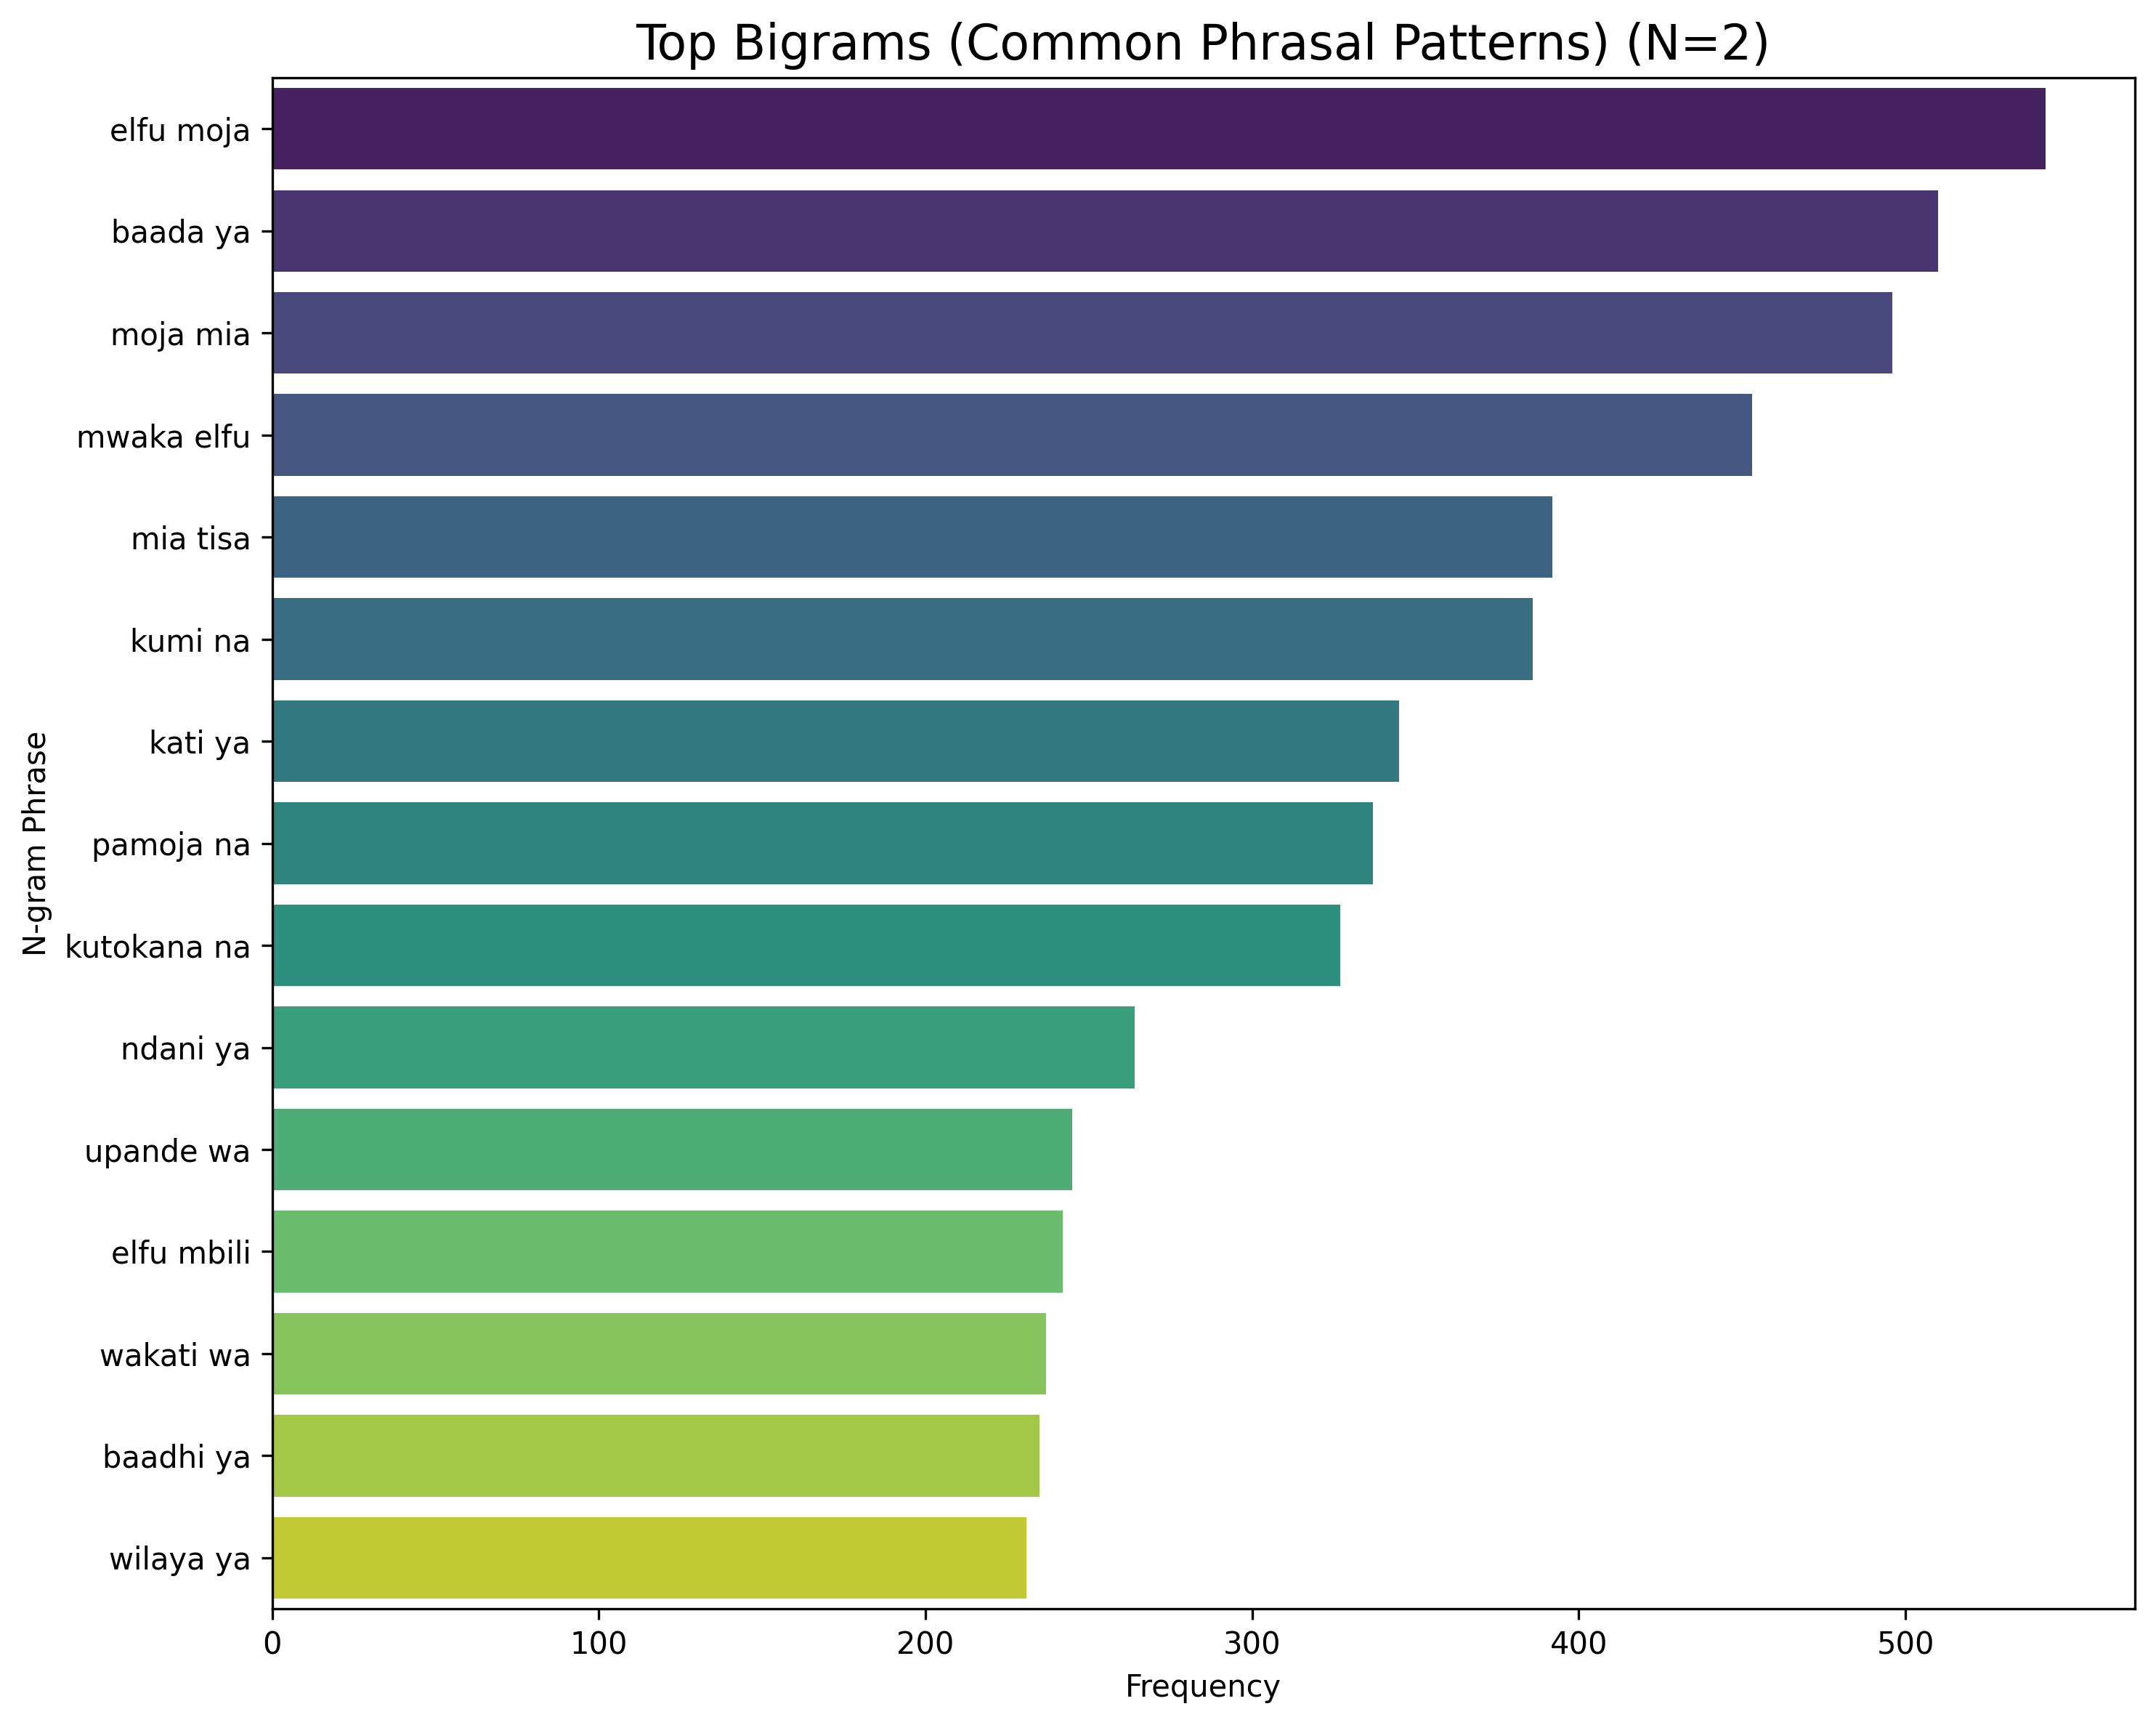
\includegraphics[width=0.6\textwidth]{images/top_bigrams_(common_phrasal_patterns).pdf}
\caption{Most frequent Swahili bigrams illustrating phrasal structure}
\label{fig:bigrams}
\end{figure}

The final assessment for completeness highlighted that columns such as "Accent" and "Segment" were entirely missing and irrecoverable. Linguistically, an audit of target sentences confirmed the presence of the phonetic apostrophe and loanword characters such as 'q' and 'x', informing the requirement for a 58-token vocabulary to ensure the ASR model captures the full semantic breadth of Kiswahili.

\subsection{Text and Unstructured Data Analytics}
This phase involves analyzing the thematic content of the corpus to justify the linguistic preprocessing required for high-accuracy NLP tasks. A critical step included the development of a custom library of Swahili stop-words, categorized into 17 linguistic groups such as \textit{Viashiria} (demonstratives), \textit{Viwakilishi} (pronouns), and \textit{Vitenzi Msaada} (auxiliary verbs). Comparing word clouds before and after stop-word removal visually demonstrates the high density of "noise" in low-resource language data, as shown in Figure~\ref{fig:wordcloud}. This thematic extraction is vital for ensuring that subsequent components, such as Sentiment Analysis and Summarization, focus on sentiment-bearing keywords and core intent rather than functional particles \citep{Banda_2012}.

\begin{figure}[h]
\centering
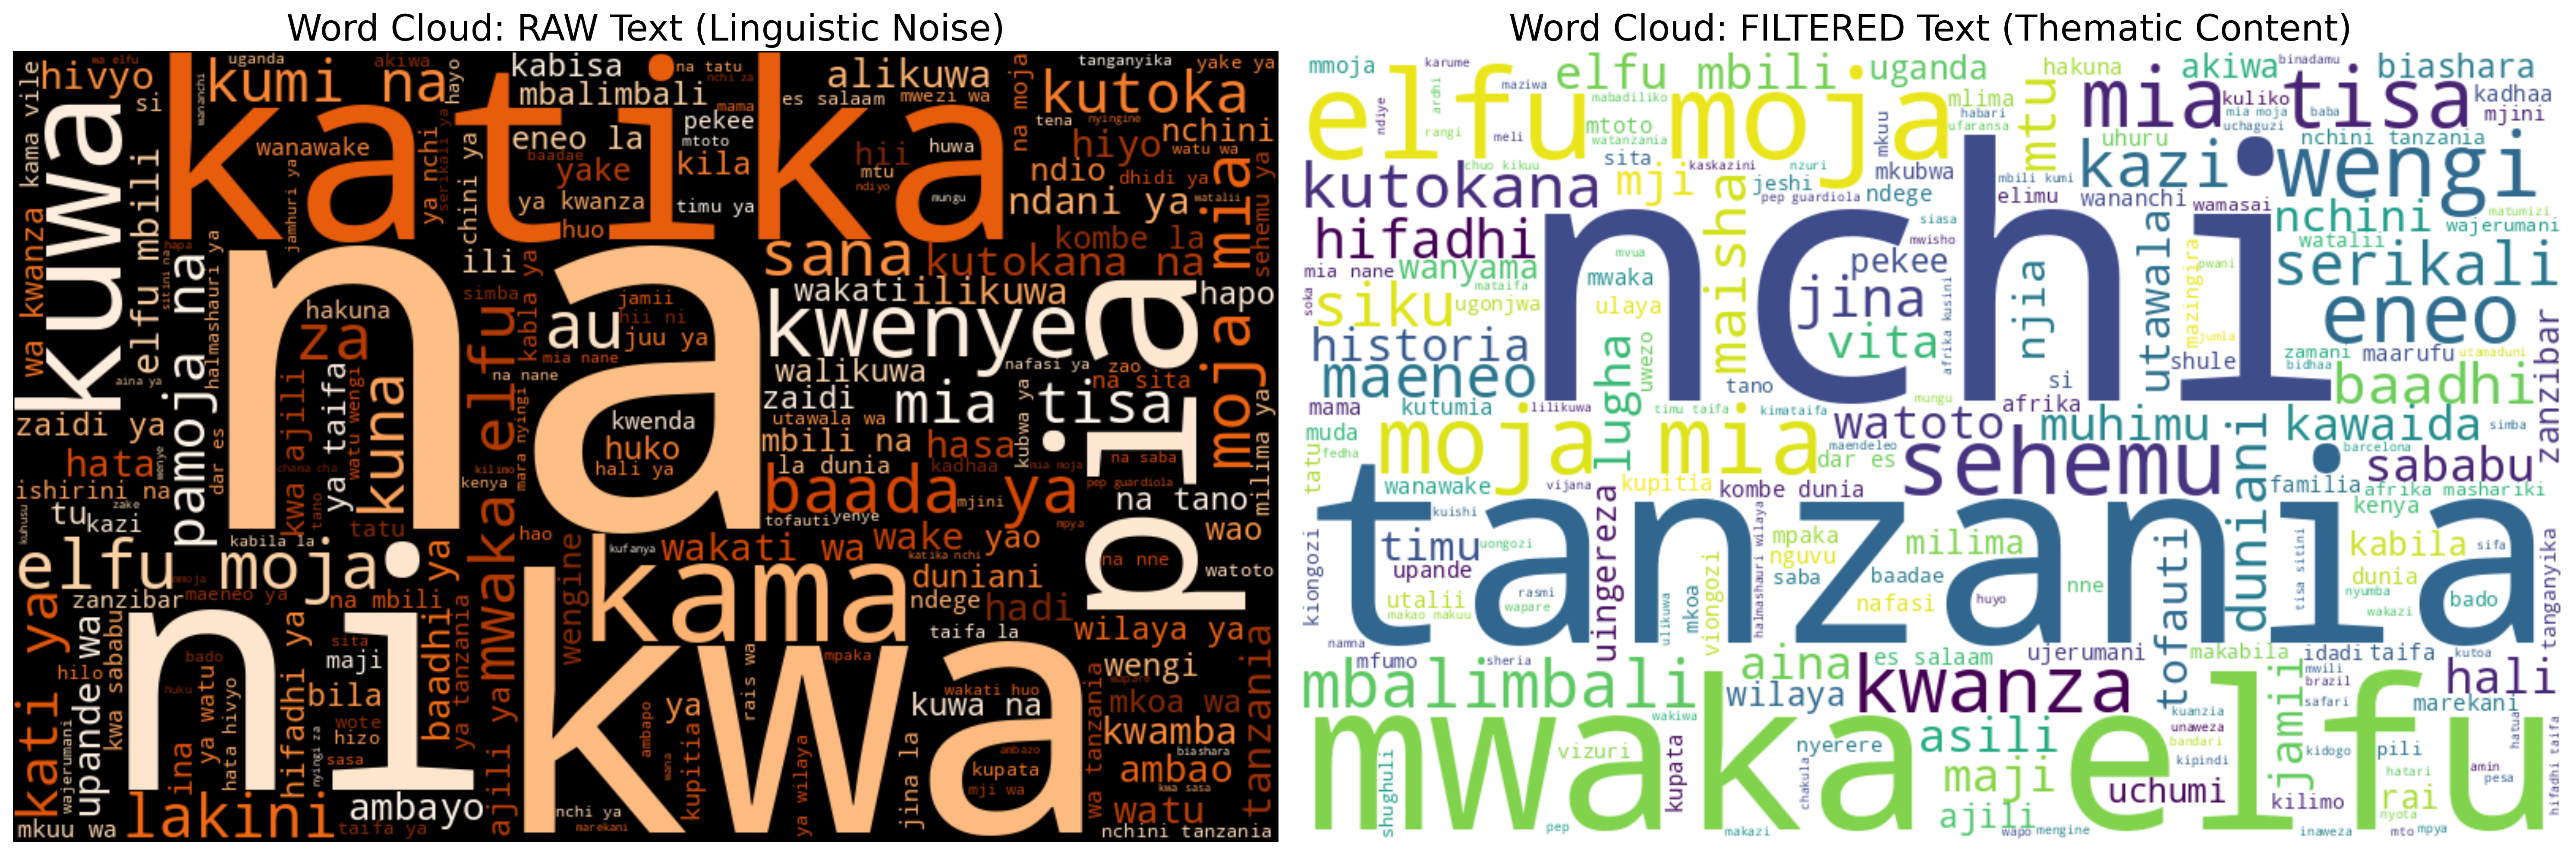
\includegraphics[width=\textwidth]{images/wordcloud_comparison.png}
\caption{Word cloud comparison before and after Swahili stop-word removal}
\label{fig:wordcloud}
\end{figure}

\noindent\textbf{Exploratory Sentiment Characterization.}

As part of the unstructured text analytics, an exploratory sentiment inference was conducted on the transcribed Kiswahili sentences to assess the affective distribution of the corpus. This analysis employed a pretrained multilingual transformer-based sentiment model applied directly to the text. The purpose of this step was not to construct a supervised sentiment classifier, but rather to characterize the emotional properties of the dataset and evaluate its suitability for downstream semantic analysis \citep{Mabokela_Ngcobo_Masala_2025, Mabokela_Celik_Raborife_2023}.

The inferred sentiment distribution revealed a strong dominance of neutral classifications, with positive and negative sentiments occurring only marginally. This outcome aligns with the functional and instructional design of the Common Voice prompts, which are primarily declarative and phonetically motivated rather than emotionally expressive. Examination of model confidence scores further indicated weak class separation, suggesting that affective cues within the corpus are sparse and contextually ambiguous.

Given the absence of ground-truth sentiment annotations and the low emotional variance observed, conventional supervised evaluation metrics such as precision, recall, and F1-score were deemed methodologically inappropriate. Consequently, the results are reported descriptively through label distributions, confidence scores, and representative example predictions. These findings confirm that sentiment analysis, while feasible as an auxiliary post-transcription task, does not constitute a reliable predictive objective for this dataset.

Importantly, the observed neutrality bias serves as an empirical validation of the corpus design and supports the exclusion of sentiment features from the core ASR training pipeline, while still permitting their optional inclusion for exploratory analysis and metadata enrichment \citep{Mabokela_Ngcobo_Masala_2025}.

\section{Data Cleaning and Preprocessing}
To ensure the accuracy, reliability, and computational efficiency of the subsequent machine learning models, the raw Kiswahili dataset underwent a comprehensive cleaning and preprocessing pipeline. This phase was designed to mitigate the inherent "noise" of crowdsourced data, reduce irrelevant computational overhead, and standardize both audio and textual inputs to facilitate effective model training. The pipeline comprised several specialized stages: audio silence trimming, spectral noise reduction, text normalization, and robust metadata validation.

\subsection{Silence Trimming}
The initial stage of audio preprocessing focused on the removal of non-informative silent segments from the temporal boundaries of each recording. Utilizing the \texttt{librosa.effects.trim()} function, the system automatically identified and removed segments where the decibel level fell below a predefined threshold as illustrated in Figure~\ref{fig:silence_trim}. 

The retention of leading or trailing silence offers no instructional value for Automatic Speech Recognition (ASR) training. These segments artificially inflate the duration of audio clips, resulting in increased processing latency and higher computational costs during the feature extraction and modeling phases. 

\begin{figure}[h]
\centering
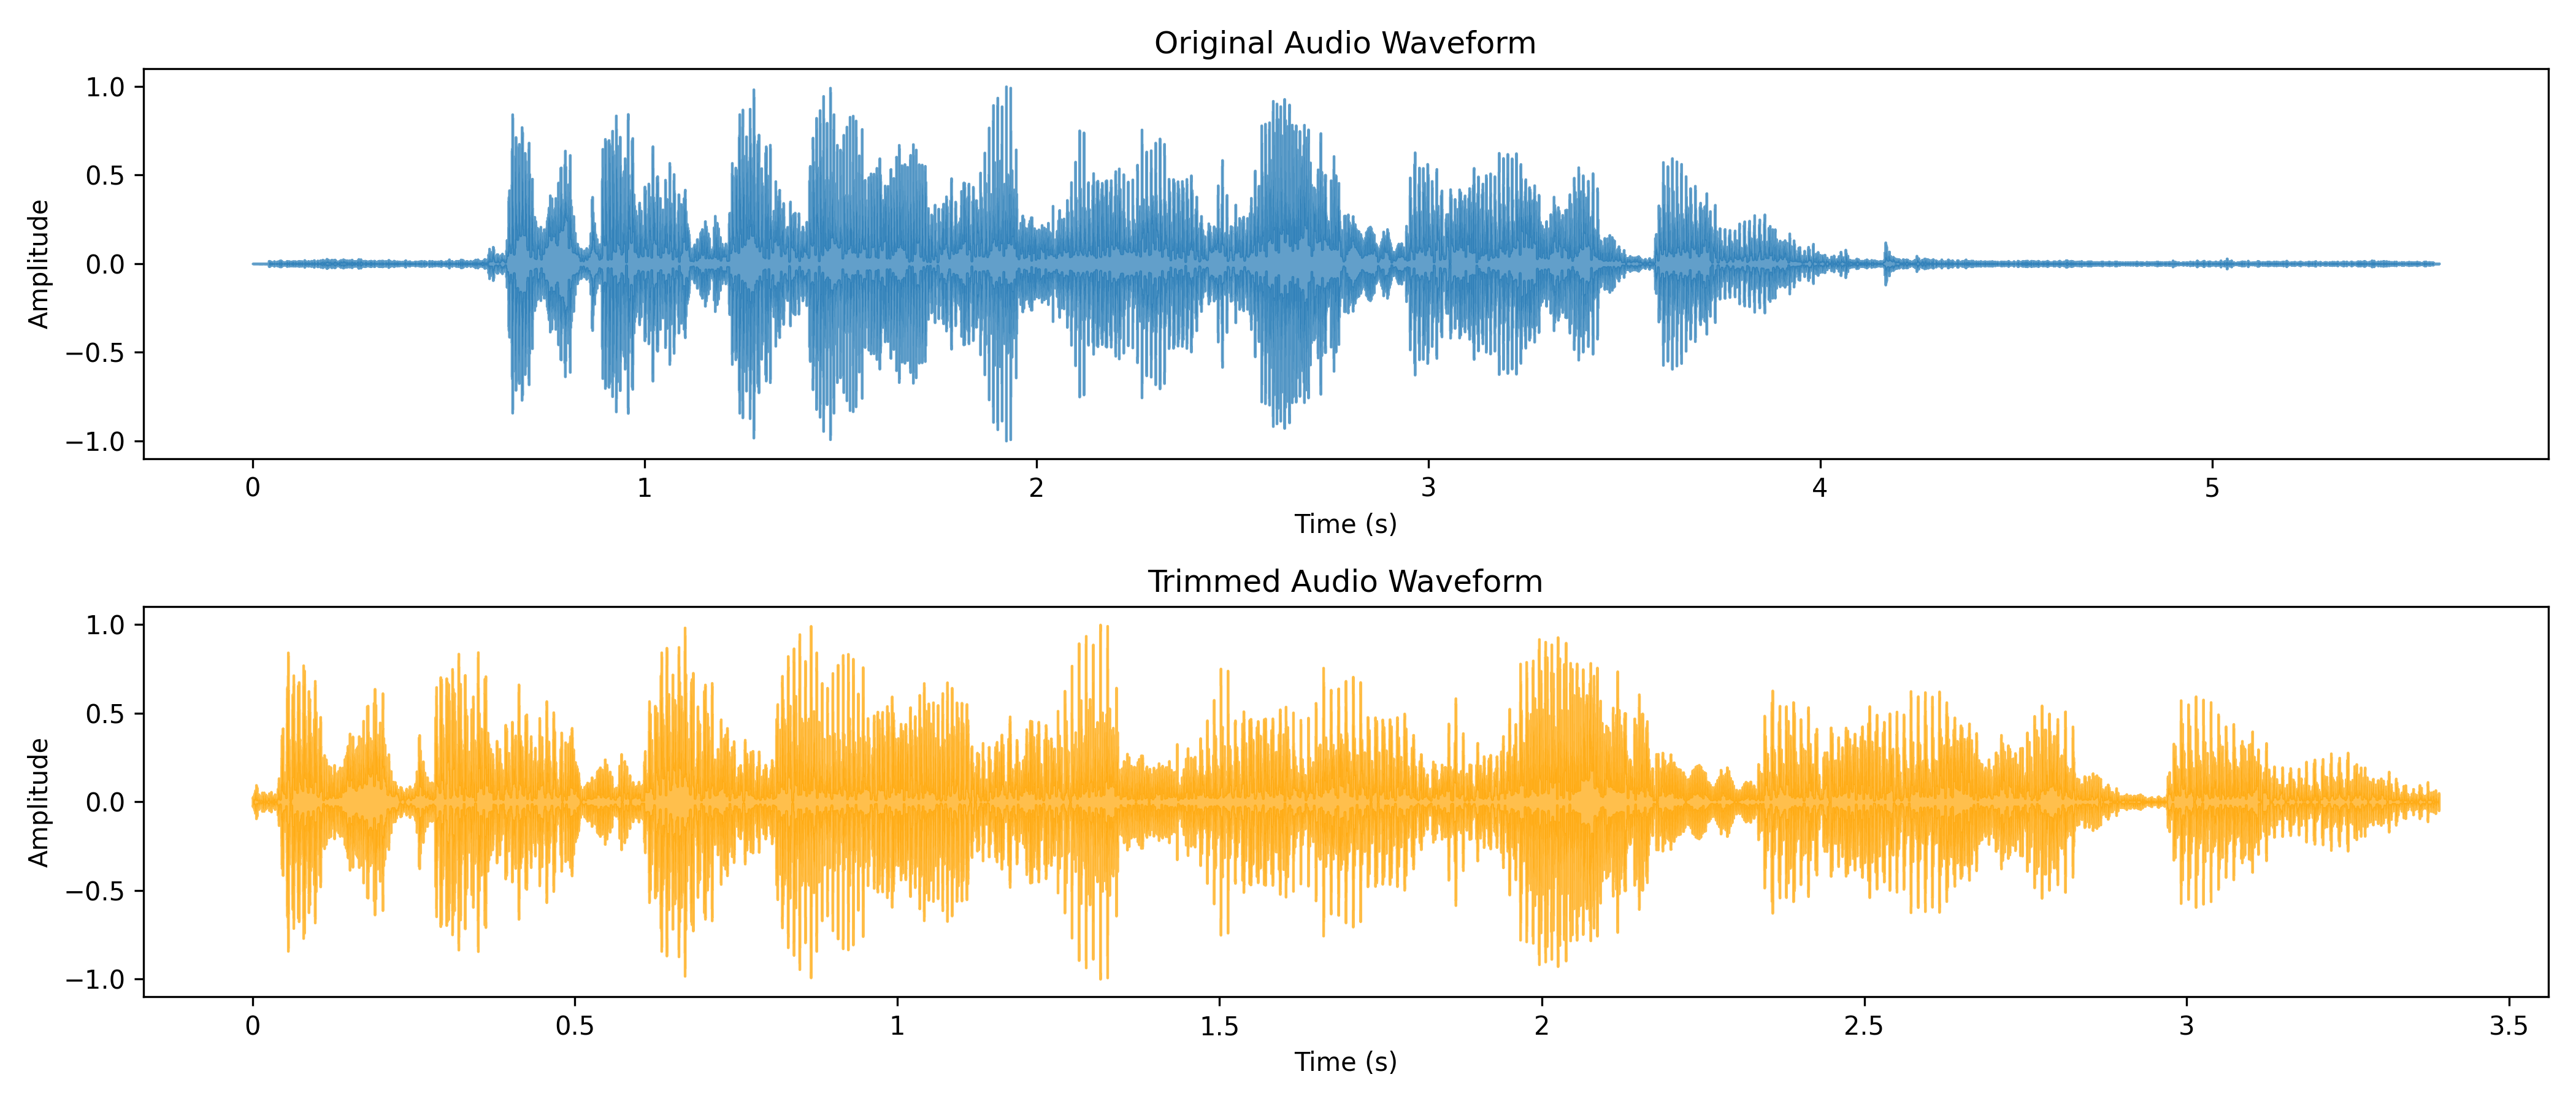
\includegraphics[width=\textwidth]{images/silence_trimming_comparison.pdf}
\caption{Waveform comparison before and after silence trimming}
\label{fig:silence_trim}
\end{figure}

Furthermore, eliminating these segments prevents the model from inadvertently learning patterns unrelated to speech, thereby reducing the risk of overfitting and enhancing the model's ability to generalize to natural, continuous speech \citep{Mueller2015}.

Mathematically, the trimming process is defined by the following energy-based selection:
\begin{equation}
\text{Trimmed Audio} = \{ \text{Audio}[t] \mid \text{Energy}(\text{Audio}[t]) > \tau \}
\end{equation}
Where:
\begin{itemize}
    \item $\text{Audio}[t]$ represents the discrete audio signal at time $t$.
    \item $\text{Energy}(\text{Audio}[t]) = |\text{Audio}[t]|^2$ represents the instantaneous energy of the signal.
    \item $\tau$ is the predefined energy threshold distinguishing active speech from background silence.
\end{itemize}

\subsection{Noise Reduction via Spectral Gating}
To enhance the clarity of the speech signal, a spectral gating algorithm was implemented using the \texttt{pydub} library \citep{jiaaro2025pydub}. Background noise, such as environmental hums or static, can significantly degrade ASR performance by creating spectral distortions that confuse the encoder during training. 

The algorithm functions by first calculating a ``noise floor'' based on the initial $1/10^{\text{th}}$ of the audio signal, assuming this segment contains only background ambient noise. Mathematically, the noise floor is derived as:
\begin{equation}
\text{Noise Floor} = \frac{1}{n} \sum_{i=1}^{n} |S(f, t)_i|
\end{equation}

where $n$ represents the number of samples in the initial segment and $|S(f, t)_i|$ is the absolute value of the $i$-th component in the spectrogram. The noise threshold is subsequently set as twice the noise floor ($\tau = 2 \times \text{Noise Floor}$). The cleaning process follows a gating logic:
\begin{equation}
S_{\text{clean}}(f, t) = 
\begin{cases} 
S(f, t) & \text{if } |S(f, t)| > \tau \\
0 & \text{if } |S(f, t)| \leq \tau 
\end{cases}
\end{equation}

A visual comparison of the spectrograms before and after noise suppression illustrates the effectiveness of this approach, as shown in Figure~\ref{fig:noise_reduction}.

\begin{figure}[H]
\centering
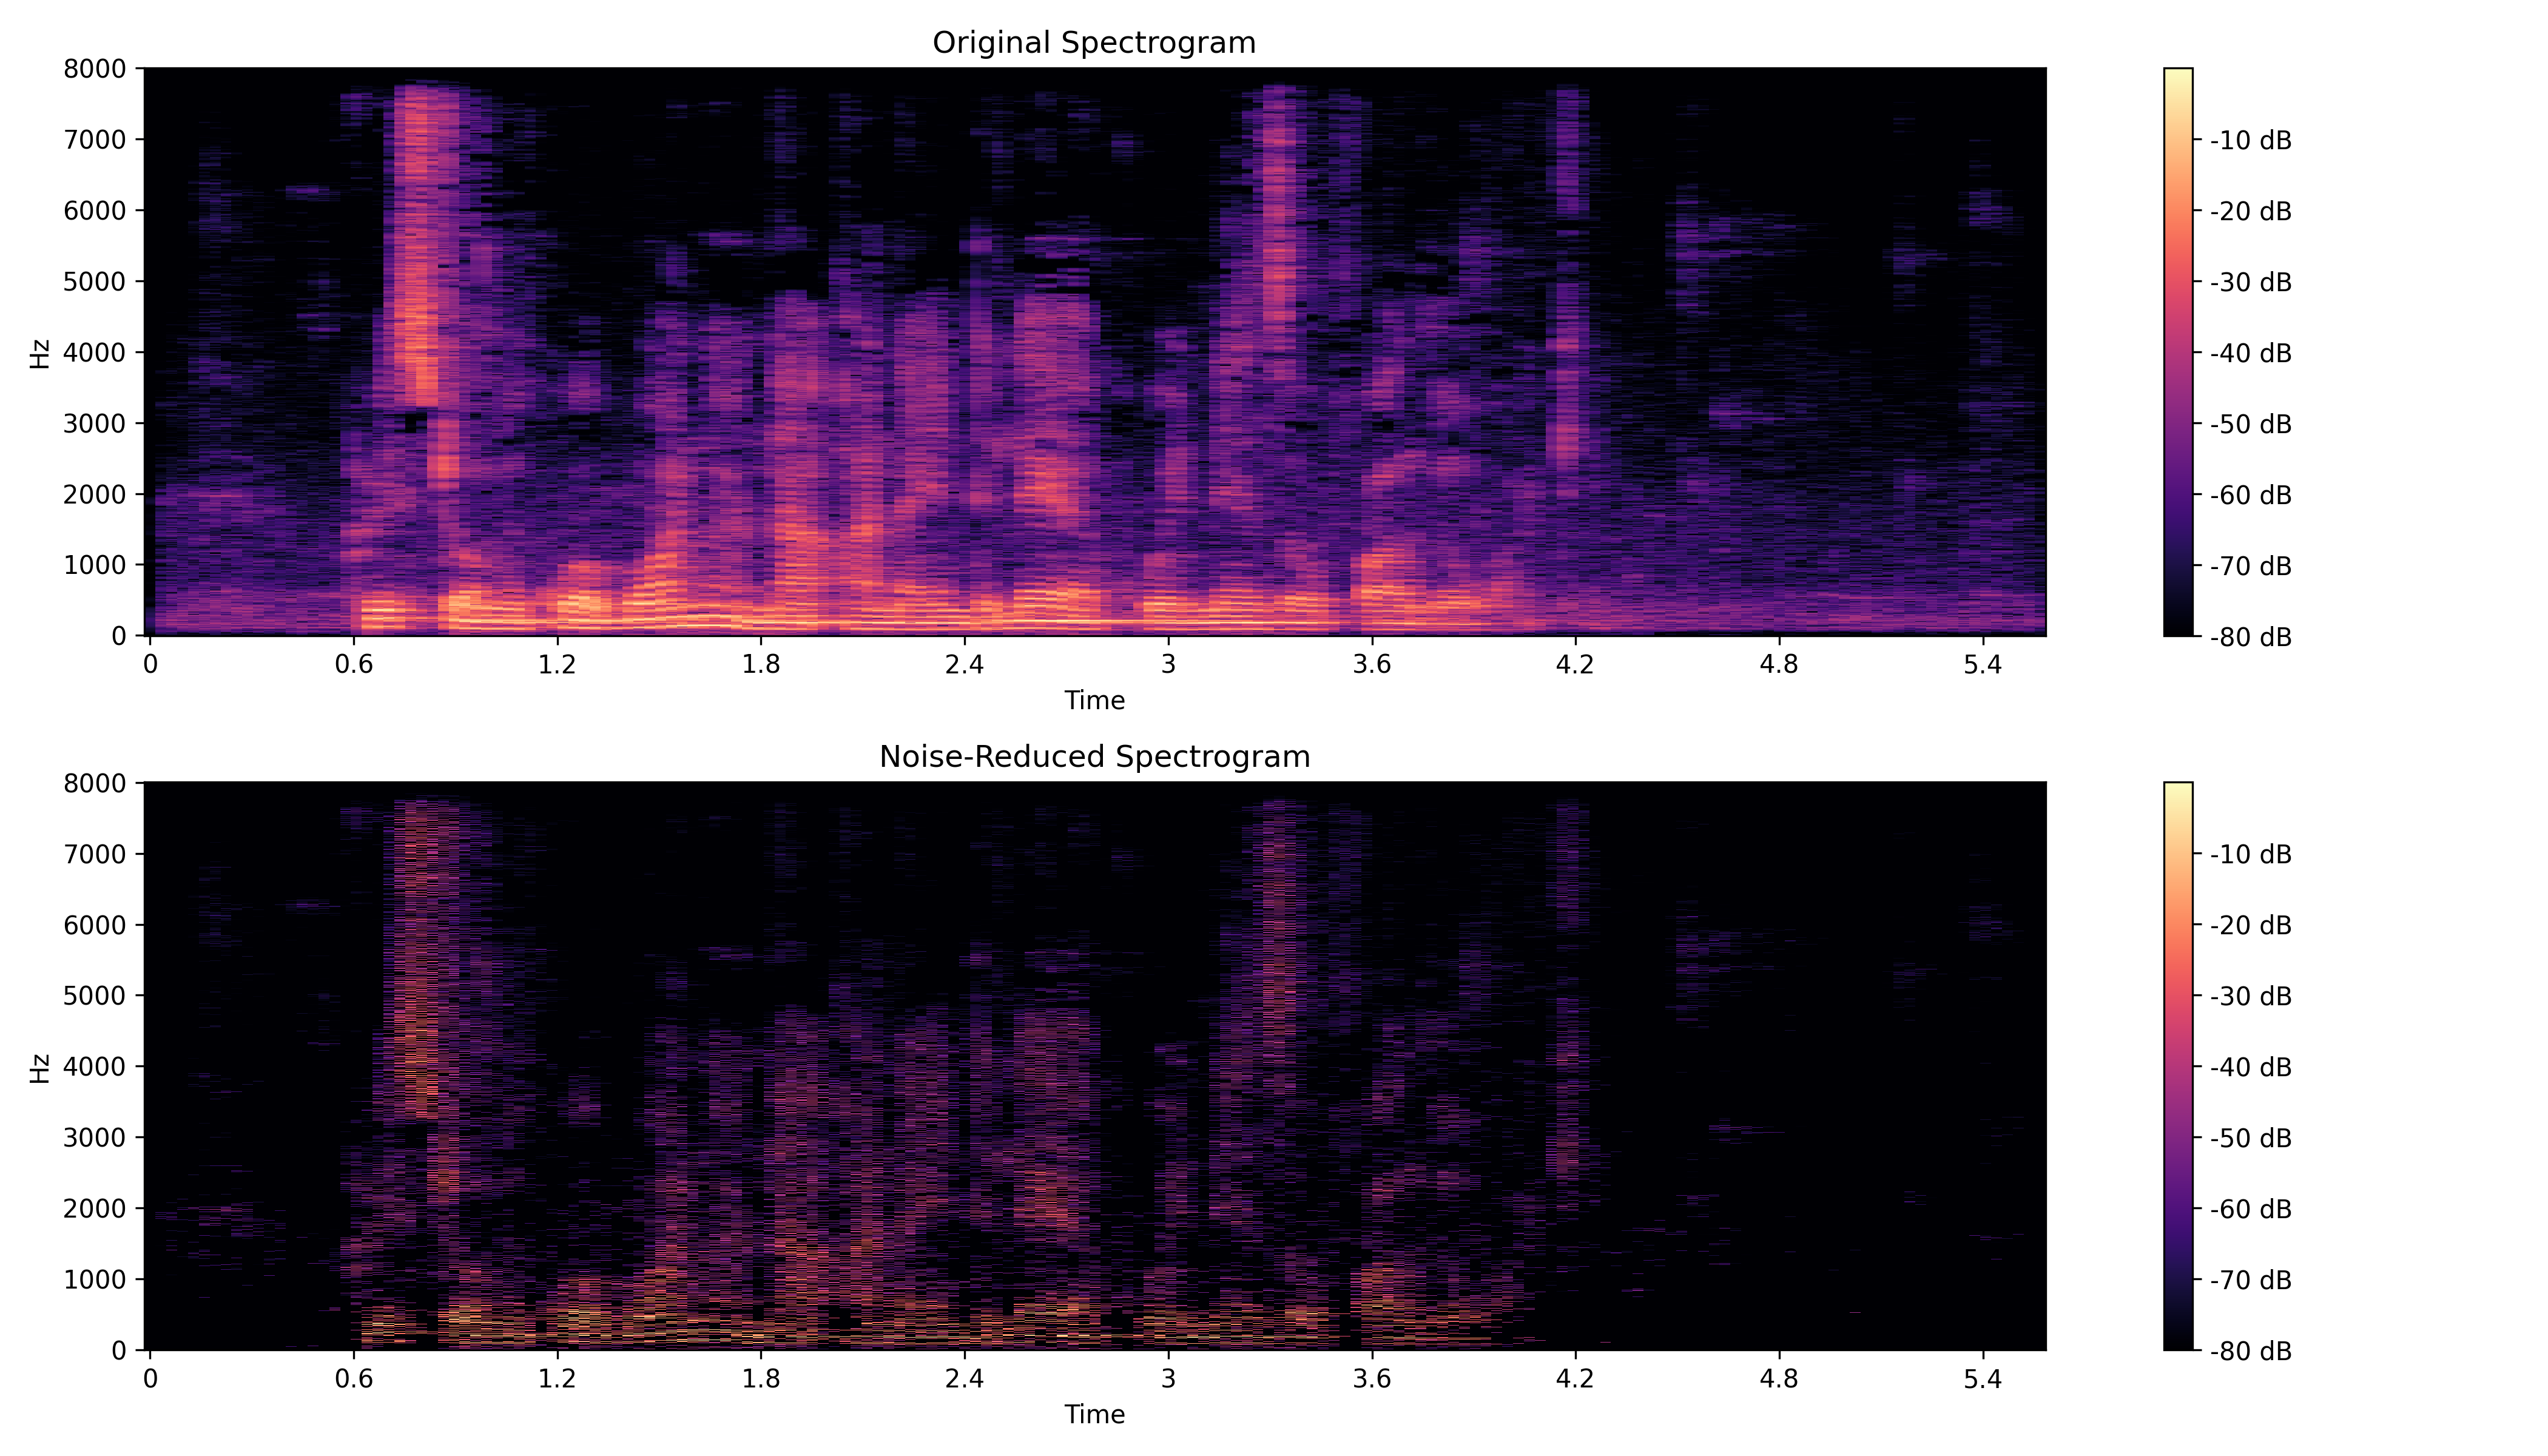
\includegraphics[width=\textwidth]{images/noise_reduction_spectrogram.pdf}
\caption{Spectrogram comparison before and after spectral noise reduction}
\label{fig:noise_reduction}
\end{figure}

This ensures that only frequency components with sufficient energy to likely represent speech are preserved, resulting in a cleaner signal that improves transcription accuracy across diverse acoustic environments.

\subsection{Text Normalization}
Text normalization was performed to standardize the linguistic targets and reduce data complexity. This step ensured the model focused on semantic patterns rather than orthographic variations. The normalization process included converting all text to lowercase and stripping non-essential punctuation. Critically, for the Kiswahili context, the phonetic apostrophe ($'$) was preserved, as it holds semantic significance. Additionally, a custom library of stop-words was utilized to prune functional particles during the sentiment analysis and summarization preparation, allowing the models to concentrate on high-entropy keywords \citep{Banda_2012, nltk2025}.

\subsection{Handling Missing Values and Metadata Validation}
Incomplete metadata poses a risk of introducing systematic bias, particularly when utilizing demographic features like age or gender for performance auditing. Rather than discarding records with missing values which would result in a loss of valuable acoustic data, this research utilized a neutral placeholder strategy. Missing categorical entries were imputed with the string "unknown" or "unspecified." This approach maintains the integrity of the total dataset, ensures uniform representation across all data points, and prevents the unjustifiable exclusion of contributors from the training set, thereby supporting a more robust and inclusive final model \citep{Nganga_Maroko_Ong_onda_2023}.

\subsection{Acoustic Feature Extraction}
Following cleaning, the audio was transformed into structured representations. Mel-Frequency Cepstral Coefficients (MFCCs) were extracted to summarize the spectral envelope most relevant to human speech perception. Additionally, Mel spectrograms were generated using a Short-Time Fourier Transform (STFT) to map the signal into a two-dimensional time-frequency representation. These features provide a critical balance between dimensionality reduction and the preservation of phonetic information required for high-accuracy ASR.

\section{Machine Learning Modeling}

The core architecture employs a suite of Transformer-based models optimized for distinct linguistic tasks. In the current study, only the ASR module is fine-tuned on the Swahili dataset, while sentiment analysis and summarization leverage pre-trained multilingual models for inference.

\subsection{Speech Recognition: Wav2Vec 2.0}
The primary engine for Automatic Speech Recognition (ASR) in this research is the \textit{"eddiegulay/wav2vec2-large-xlsr-mvc-swahili"} model \citep{eddiegulay2021wav2vec2}. This architecture represents a sophisticated application of the Wav2Vec 2.0 framework, specifically fine-tuned for the phonetic and morphological nuances of the Swahili language. The model is built upon the Cross-lingual Speech Representations (XLSR) approach, which leverages large-scale pre-training on thousands of hours of multilingual speech to learn a universal acoustic subspace \citep{baevski2020wav2vec20frameworkselfsupervised}.

The learning objective of this model is centered on a self-supervised contrastive task. It is optimized by minimizing a contrastive loss function ($\mathcal{L}_{\text{ASR}}$), which forces the model to distinguish a true quantized latent speech representation from a set of negative ``distractor'' samples within a shared embedding space. This is mathematically expressed as:

\begin{equation}
    \mathcal{L}_{\text{ASR}} \propto - \log \frac{e^{\text{sim}(\mathbf{z}_v, \mathbf{c}_v) / \kappa}}{\sum_{\tilde{\mathbf{z}} \in \mathbb{Z}} e^{\text{sim}(\tilde{\mathbf{z}}, \mathbf{c}_v) / \kappa}}
\end{equation}

where $\mathbf{z}_v$ denotes the predicted quantized latent representation at time $v$, $\mathbf{c}_v$ represents the true context representation generated by the Transformer layers, $\text{sim}$ computes the cosine similarity between these vectors, $\kappa$ is a constant temperature scaling factor, and $\mathbb{Z}$ represents the union of the true target and $K$ distractor representations.

The implementation of this specific model provides several critical advantages for Swahili speech analysis:
\begin{itemize}
    \item \textbf{Cross-Lingual Transfer Learning:} As Swahili is a low-resource language regarding high-fidelity labeled acoustic data, the XLSR-based variant is essential. It enables the system to benefit from acoustic patterns learned from high-resource languages, significantly improving the recognition of Swahili phonemes even with limited native training data \citep{eddiegulay2021wav2vec2}.
    
    \item \textbf{Raw Waveform Feature Extraction:} Unlike traditional ASR systems that rely on manually engineered features like Mel-frequency cepstral coefficients (MFCCs), Wav2Vec 2.0 utilizes a multi-layer convolutional neural network (CNN) as a feature encoder. This allows the model to process raw audio waveforms directly, capturing fine-grained temporal and spectral details that are typically lost in standard spectrogram conversions \citep{baevski2020wav2vec20frameworkselfsupervised}.
    
    \item \textbf{Contextual Modeling via Transformers:} Following feature extraction, a deep Transformer architecture is utilized to capture long-range dependencies in the speech signal. This is vital for Swahili, where word meaning is heavily dependent on agglutinative structures such as prefixes and suffixes.
    
    \item \textbf{Connectionist Temporal Classification (CTC):} The model employs a CTC decoding head to map continuous audio signals to discrete text characters. This facilitates an ``end-to-end'' training approach that does not require the audio to be pre-aligned with the transcript, streamlining the inference pipeline for real-world Swahili dialogue.
\end{itemize}

This strategic choice of the Wav2Vec 2.0 architecture ensures that the system achieves high transcription accuracy even in the presence of varying accents and background noise, ultimately resulting in a robust foundation for downstream exploratory semantic analysis and abstractive summarization \citep{DHAHBI2025100615}.

\subsection{Sentiment Analysis: DistilBERT(Pre-trained)}
For exploratory semantic characterization of the transcribed output, the system applies a pretrained multilingual sentiment inference model, specifically \textit{"lxyuan/distilbert-base-multilingual-cased-sentiments-student"}. 

Unlike the ASR components, this module is not trained or fine-tuned within this research and does not rely on ground-truth sentiment annotations. Instead, it operates as a zero-shot, model-inferred analytical layer used to assess whether affective signals are meaningfully present in the automatically generated Swahili transcripts.

While the underlying model was originally optimized using a Cross-Entropy Loss function ($\mathcal{L}_{\text{Sentiment}}$) during its pretraining phase \citep{Kumar_Deep_Kalra_2024}, no supervised loss optimization was performed in this study. The model was used strictly in inference mode to generate probabilistic sentiment distributions over predefined classes, which were subsequently analyzed descriptively rather than evaluated against labeled ground truth.

\begin{equation}
    \mathcal{L}_{\text{Sentiment}} = - \frac{1}{N} \sum_{i=1}^{N} \sum_{c=1}^{C} y_{i,c} \log(\hat{y}_{i,c})
\end{equation}

where $N$ denotes the total number of samples, $C$ represents the number of sentiment classes, $y_{i,c}$ is a binary indicator (0 or 1) if class label $c$ is the correct classification for observation $i$, and $\hat{y}_{i,c}$ is the predicted probability of observation $i$ belonging to class $c$.

The selection of this "student" distilled model over larger, more traditional architectures such as BERT-Large or RoBERTa is justified by several critical technical factors essential for a real-time Swahili ASR pipeline:

\begin{itemize}
    \item \textbf{Knowledge Distillation Efficiency:} This model utilizes a teacher-student framework where a smaller model (the student) is trained to reproduce the behavior of a larger, more complex model (the teacher). This results in a model that retains approximately 97\% of the teacher's performance while being 40\% smaller and 60\% faster, making it ideal for deployment on hardware with limited resources, such as CPUs \citep{wolf2020huggingfacestransformersstateoftheartnatural}.
    
    \item \textbf{Multilingual Generalization:} Unlike English-centric sentiment models, the cased multilingual nature of this model allows it to handle the nuances of Swahili text. It effectively processes capital letters and regional phonetic markers which are crucial for maintaining semantic context in low-resource linguistic environments \citep{Kumar_Deep_Kalra_2024}.
    
    \item \textbf{Inference Latency Reduction:} In a production environment using FastAPI, the bottleneck is often the acoustic model. By utilizing a "student" DistilBERT, we minimize the overhead of the sentiment head, allowing the system to process transcripts nearly instantaneously without increasing the total end-to-end response time \citep{Bodor_Hnida_Daoudi_2023}.
    
    \item \textbf{Robustness to Noisy Transcripts:} Student models often exhibit better generalization when faced with slightly imperfect transcripts, such as those generated in ASR tasks, as they focus on the most significant semantic features learned from the teacher model rather than overfitting to specific training noise \citep{Wu_Jin_Shi_Liang_Zhan_2024}.

    \item \textbf{Exploratory Role in the Pipeline:} Sentiment inference was treated as a diagnostic and descriptive component rather than a predictive objective. Observed class distributions and confidence scores were used to assess corpus characteristics and to inform downstream analytical decisions, not to optimize or validate model performance \citep{Mabokela_Ngcobo_Masala_2025}.
\end{itemize}

This strategic choice ensures that the final system provides high-fidelity sentiment classification while maintaining the high performance required for real-world application.

\subsection{Text Summarization: mT5-small (Pre-trained)}
The final stage of the linguistic processing pipeline involves abstractive summarization using the \textit{google/mt5-small} model. This architecture is based on the Text-to-Text Transfer Transformer (T5) framework, which conceptualizes every Natural Language Processing (NLP) task, including summarization as a sequence-to-sequence mapping problem \citep{DHAHBI2025100615}. 

The model was not fine-tuned on the Swahili dataset due to the failure of training attempts on noisy ASR transcripts. Instead, zero-shot summarization is used for exploratory text summarization of the transcriptions. The model is optimized by generating the correct target summary tokens, which involves minimizing a sequence-to-sequence loss function ($\mathcal{L}_{\text{T5}}$):

\begin{equation}
    \mathcal{L}_{\text{T5}} = - \sum_{t} \log P(\mathbf{y}_t^* \mid \mathbf{y}_{<t}^*, \mathbf{x}; \theta)
\end{equation}

In this equation, $\mathbf{y}_t^*$ represents the ground-truth target token at time step $t$, $\mathbf{y}_{<t}^*$ denotes the sequence of tokens generated in previous steps, $\mathbf{x}$ is the input Swahili transcription, and $\theta$ represents the trainable model parameters \citep{DHAHBI2025100615}.

The selection of the \textit{mT5-small} variant for this research is justified by several comprehensive technical considerations:

\begin{itemize}
    \item \textbf{Massively Multilingual Pre-training:} Unlike the standard T5 model, which is primarily trained on English datasets (C4), the mT5 model is pre-trained on the mC4 corpus, which encompasses over 101 languages, including Swahili. This cross-lingual pre-training allows the model to leverage "transfer learning" from high-resource languages to effectively understand the syntax and semantics of Swahili, despite it being a lower-resource language in the digital domain.
    
    \item \textbf{Abstractive Summarization Capability:} By treating summarization as conditional text generation, the model can produce novel, grammatically correct Swahili sentences that capture the core meaning of the transcript, rather than relying solely on extractive methods.
    
    \item \textbf{Computational Efficiency and Deployment:} The "small" variant of mT5 was specifically chosen to balance linguistic capability with deployment feasibility. With approximately 300 million parameters, the model is significantly more lightweight than its \texttt{base} or \texttt{large} counterparts. This reduction in parameter count is critical for minimizing the memory footprint and inference latency when hosted within a FastAPI backend on standard CPU-based server environments \citep{DHAHBI2025100615}.
    
    \item \textbf{Byte-Level Byte-Pair Encoding (BBPE):} mT5 utilizes a specialized tokenizer that employs byte-level fallback. This is particularly important for Swahili ASR outputs, as it prevents the generation of "unknown" (\texttt{[UNK]}) tokens when encountering rare phonetic spellings or regional dialects, ensuring that the generated summary remains readable and semantically coherent.
\end{itemize}

By integrating the mT5 model into the pipeline, the system transforms raw, potentially long-winded spoken dialogue into concise, actionable intelligence, fulfilling the research objective of providing an end-to-end analytical tool for Swahili speech.

\subsection{Performance Evaluation Metrics}
The overall effectiveness of the proposed pipeline is quantified using standard evaluation metrics appropriate to each module. Given the end-to-end nature of the system, metrics were selected to reflect the performance of both transcription and summarization tasks, while sentiment analysis is treated as exploratory.

\textbf{Word Error Rate (WER)}

The ASR component is evaluated using the Word Error Rate (WER), a standard metric that quantifies the discrepancy between predicted transcripts and reference text. WER is calculated as:

\begin{equation}
    \text{WER} = \frac{S + D + I}{N}
\end{equation}

where:
\begin{itemize}
    \item $S$ denotes the number of \textit{substitutions},
    \item $D$ denotes the number of \textit{deletions},
    \item $I$ denotes the number of \textit{insertions}, and
    \item $N$ represents the total number of words in the reference transcript.
\end{itemize}

WER provides a robust measure of transcription accuracy, capturing the cumulative effect of misrecognitions, missing words, and spurious insertions. A lower WER indicates higher fidelity in the ASR output, which is critical for downstream tasks such as summarization and sentiment analysis \citep{DHAHBI2025100615}.

\textbf{ROUGE and BLEU Scores}

Summarization performance is evaluated using ROUGE-N metrics and the BLEU score. ROUGE-N measures n-gram overlap between generated summaries and reference summaries, reflecting content coverage, while BLEU assesses the fluency and lexical similarity of the generated text:

\begin{equation}
    \text{BLEU} = \text{BP} \cdot \exp\left(\sum_{n=1}^{N} w_n \log p_n\right)
\end{equation}

where $p_n$ is the precision of n-grams of size $n$, $w_n$ is the weighting for each n-gram, and $\text{BP}$ is the \textit{Brevity Penalty}, applied to penalize overly short summaries and ensure semantic completeness.

Due to the failure of fine-tuning mT5 on noisy ASR transcripts, ROUGE and BLEU metrics are reported only as exploratory indicators. They provide a reference for the alignment between generated summaries and expected semantic content, but should not be interpreted as conclusive performance evidence \citep{DHAHBI2025100615}.

\textbf{Sentiment Analysis Metrics}

Sentiment analysis results are intentionally \textit{not} included in conventional quantitative metrics such as accuracy or F1-score. The inferred labels are exploratory, serving to provide insights into the emotional tone of transcribed speech rather than ground truth classification. Evaluation focused on:
\begin{itemize}
    \item \textbf{Label Distribution:} Frequency of positive, neutral, and negative predictions across transcripts.
    \item \textbf{Confidence Scores:} Model-provided probability scores to gauge reliability of predictions.
    \item \textbf{Qualitative Inspection:} Manual review of representative transcripts to assess semantic coherence and sentiment alignment \citep{Mabokela_Ngcobo_Masala_2025}.
\end{itemize}

This evaluation strategy aligns with the exploratory role of sentiment analysis in the pipeline, providing actionable insights without over-interpreting model outputs.

\section{Deployment}
\label{sec:technical_architecture}

This section presents a comprehensive technical documentation of the deployed Kiswahili audio processing system. The architecture is designed to operationalize the models developed in earlier phases of the CRISP-DM framework and to demonstrate their applicability in a real-world, end-to-end deployment context. Emphasis is placed on modularity, scalability, robustness, and reproducibility to ensure that the system functions as both a research prototype and a foundation for future production-level extensions.

\subsection{System Architecture Overview}

The system follows a modular, service-oriented architecture that separates concerns across clearly defined components. Each module encapsulates a specific responsibility, enabling independent development, testing, and maintenance. This design choice improves system maintainability and allows individual components, such as the ASR model or sentiment analysis module to be replaced or upgraded without affecting the overall pipeline.

At a high level, the system consists of three primary layers:
\begin{itemize}
    \item A \textbf{web-based frontend} responsible for user interaction and result visualization.
    \item A \textbf{FastAPI-based backend} that orchestrates processing and exposes a unified API endpoint.
    \item A \textbf{machine learning pipeline layer} that performs speech recognition, sentiment analysis, and summarization.
\end{itemize}

The directory structure reflects this modular philosophy and is documented to support reproducibility and clarity for future researchers.

\subsection{Processing Flow Architecture}

\begin{figure}[H]
    \centering
    \includegraphics[width=\textwidth]{images/processing_flow_architecture.drawio.pdf}
    \caption{End-to-end processing flow architecture of the Kiswahili audio pipeline}
    \label{fig:processing_flow}
\end{figure}


Figure~\ref{fig:processing_flow} conceptually illustrates the request processing pipeline. Upon receiving an audio input, the system first evaluates the audio duration to determine the appropriate processing strategy. Short audio segments are processed directly, while longer recordings are segmented using an overlapping chunking strategy to ensure that model input constraints are respected without losing contextual continuity.

Following transcription, the resulting text undergoes a secondary validation based on token length. If the transcription exceeds the maximum token limit supported by downstream transformer models, sentence-aware text chunking is applied. This ensures that both sentiment analysis and summarization can be performed reliably without truncation or semantic distortion.

The final stage aggregates outputs from all intermediate components into a single structured JSON response returned to the frontend.

\subsection{Backend Architecture Using FastAPI}

The selection of FastAPI for backend implementation is grounded in its high performance, asynchronous request handling, and comprehensive support for automatic API documentation through OpenAPI and Swagger UI. Such attributes significantly enhance both development and testing processes, facilitating seamless user interaction with the system during its evaluation phase.

\textbf{High Performance and Asynchronous Handling}

FastAPI is designed specifically for creating high-performance APIs, leveraging Python's asynchronous programming capabilities. A recent study highlighted that FastAPI consistently outperforms many of its competitors, especially when handling numerous concurrent requests \cite{10.35784/jcsi.7738}. This parallel processing is crucial in environments demanding efficient request handling, optimizing resource use during peak workloads. Additionally, its design allows for rapid application development, which is essential for agile software environments \cite{10.1016/j.heliyon.2024.e40855}.

\textbf{Automatic API Documentation}

Another notable feature of FastAPI is its automatic generation of API documentation through OpenAPI and Swagger UI, which upholds the standards of RESTful services. This capability allows developers to interactively explore API endpoints and data types without requiring extensive manual documentation. By integrating these specifications, FastAPI saves time and reduces the likelihood of discrepancies between documentation and API implementation \cite{10.55041/ijsrem35726}. The effectiveness of this feature has been corroborated in various contexts, where FastAPI has been shown to handle complex API structures efficiently while maintaining user-friendly documentation \cite{10.25236/ajets.2023.061118}.

\textbf{Transparent Interaction During Evaluation}

The combination of high-performance capabilities and automatic documentation fosters an environment conducive to transparent evaluations of the implemented system. Developers can easily validate API responses against documented endpoints, facilitating debugging and client-side integration during testing phases \cite{10.31315/telematika.v21i1.13259}. Furthermore, FastAPI's integration with key technologies like Pydantic and Starlette enhances performance and data validation standards. Its unique approach accelerates development times while ensuring that testing processes are robust and thorough, aligning with best practices in software engineering \cite{10.55041/ijsrem35726}.

FastAPI emerges as a premier choice for backend development due to its high-performance characteristics, native support for comprehensive API documentation, and capabilities that enhance interaction during evaluation. As software engineering continues to evolve, such features will be pivotal in developing flexible and efficient backend systems.

A single unified API endpoint is exposed to the frontend. This endpoint accepts an audio file through an HTTP POST request and coordinates the full processing workflow in a strictly defined sequence:
\begin{enumerate}
    \item \textbf{Audio Input Handling}: The backend validates and temporarily stores the uploaded audio file.
    \item \textbf{Audio-to-Text Transcription}: The audio is processed using either a fine-tuned Wav2Vec2 model or the Whisper model, depending on configuration or user selection.
    \item \textbf{Sentiment Analysis}: The transcribed text is passed to a multilingual DistilBERT-based classifier to infer sentiment polarity and confidence.
    \item \textbf{Text Summarization}: In parallel, the transcription is summarized using a T5-based abstractive summarization model.
    \item \textbf{Response Generation}: All outputs are aggregated into a structured JSON object and returned to the client.
\end{enumerate}

Asynchronous execution is employed wherever possible to ensure efficient handling of concurrent requests.

\subsection{Machine Learning Pipeline Integration}
The integration of machine learning models within a coherent architecture is crucial for effective processing, manipulation, and deployment of data-driven applications. This integration often utilizes transformer-based models structured in a sophisticated, sequential yet loosely coupled pipeline. The architectural design incorporates a centralized pipeline manager responsible for initializing models, routing data between components, and ensuring efficient management of intermediate representations.

\textbf{Centralized Pipeline Management}

A centralized management approach plays a pivotal role in orchestrating actions across the various components of the machine learning pipeline. By managing model initialization and data routing, the pipeline manager facilitates a seamless workflow, allowing for easy modifications to the architecture. Such flexibility supports the introduction of new models, such as replacing existing sentiment analysis components or adding tasks like topic classification, without necessitating extensive reengineering of the foundational structure \cite{10.1038/s41467-023-44599-9}. This adaptability is crucial in dynamic development environments where requirements frequently evolve \cite{SIM20242959}.

\textbf{Resource Usage and Performance}

Resource usage analysis of the combined pipeline indicates an approximate memory requirement of 900 MB and an average end-to-end inference latency of about five seconds on CPU-based deployments. The latency can be further mitigated by leveraging GPU acceleration, which significantly enhances performance for computation-intensive tasks \cite{10.36948/ijfmr.2024.v06i05.29550}. Such performance metrics are essential for evaluating the feasibility of deploying complex machine learning systems in real-world applications where speed and efficiency are critical \cite{bdcc3020028}.

\textbf{Chunking Algorithm Design}

To effectively manage long-form audio and text inputs, the system incorporates specialized chunking algorithms designed to maintain continuity and coherence across segments. Audio chunking uses overlapping sliding windows to ensure linguistic continuity, whereas text chunking respects sentence boundaries, preventing fragmentation of semantic units \cite{Ma2023AnIF}. This dual-level strategy addresses the inherent limitations regarding input length in transformer models and is crucial for producing meaningful, aggregated outputs from segmented data \cite{SIM20242959}.

\textbf{API and Data Flow Design}

The design of the API adheres strictly to RESTful principles and employs Pydantic models to enforce input and output schemas. This ensures data consistency across different components of the architecture, simplifying frontend integration and enhancing overall system reliability \cite{10.1016/j.heliyon.2024.e40855}. Emphasizing strict schema adherence not only mitigates errors during data exchanges but also facilitates user interactions with the system, ultimately enriching the user experience \cite{10.25236/ajets.2023.061118}.

The overall data flow can be summarized as follows:

\begin{figure}[H]
    \centering
    \includegraphics[width=\textwidth]{images/APIFLOW.pdf}
    \caption{API and Data Flow Design}
    \label{fig:design_flow}
\end{figure}

\begin{quote}
Raw Audio $\rightarrow$ Validation $\rightarrow$ Chunking (if required) $\rightarrow$ ASR $\rightarrow$ Text Processing $\rightarrow$ Sentiment and Summarization $\rightarrow$ Aggregation $\rightarrow$ JSON Response
\end{quote}

This linear yet flexible flow supports both short and long audio inputs without requiring manual intervention.

The integration of transformer-based models within a well-managed pipeline, enhanced by appropriate chunking algorithms and robust API designs, exemplifies a sophisticated approach to machine learning architecture. This structure is flexible enough to accommodate changes and performance optimizations, making it suitable for a variety of applications in data processing and analysis.

\subsection{Error Handling and Robustness}
The implementation of robust error handling mechanisms is crucial in ensuring that machine learning pipelines can gracefully degrade in the presence of failures. By capturing model loading errors, invalid inputs, and runtime exceptions, the system translates these issues into informative error responses. This approach enables the pipeline to return partial results when feasible, rather than terminating completely. In cases where sentiment analysis fails, the system defaults to providing a neutral sentiment classification along with transcription and summary outputs. Such flexibility in error management is essential for maintaining user trust and operational continuity in production environments \cite{10.26615/978-954-452-049-6_084}.

\subsection{Scalability and Performance}
To tackle high-demand scenarios, the system is structured to support horizontal scaling through multiple FastAPI worker processes. The stateless architecture allows for effective deployment behind load balancers, facilitating scalability. Performance enhancements are achieved through persistent model caching, optional batch processing of data chunks, and support for GPU acceleration \cite{Inoue_2021}. Leveraging GPU capabilities is particularly important, as it allows for the processing of multiple jobs concurrently, thereby enhancing throughput while managing resource consumption more effectively \cite{li2017gpuoutperformingfpgaacceleratorarchitecture}.

Optimizing performance requires careful consideration of various factors, including memory management and caching strategies. By implementing these optimizations, the system achieves efficient deployment even on modest hardware configurations while still providing the extensibility needed for larger infrastructures \cite{Hazarika2020SurveyOM}.

\subsection{Frontend Design and User Interaction}
The frontend of the application is crafted as a lightweight and responsive web interface that empowers users to upload or record audio from their devices. By utilizing asynchronous HTTP requests to communicate with the backend, the frontend facilitates an interactive user experience, presenting transcription, sentiment analysis results, and summaries in a user-friendly manner. Abstracting the technical complexities behind a simple interface is vital for demonstrating the practical utility of the system beyond experimental settings \cite{10.25236/ajets.2023.061118}.

This frontend integration with a robust backend system not only validates the system's operational capabilities but also highlights the importance of usability in the context of machine learning applications. Ensuring a clear presentation of results fosters user engagement and confidence in the technology \cite{10.7240/jeps.683952}.

\subsection{Deployment Within the CRISP-DM Framework}
Under the CRISP-DM framework, deployment constitutes the final phase where analytical models transition into actionable systems. The creation of a functional prototype, which harmonizes all developed models into a cohesive pipeline, exemplifies this transition. This deployed system serves as a proof of concept that demonstrates technical viability while simultaneously establishing a solid groundwork for future research initiatives, user studies, and evaluations in real-world scenarios \cite{10.1145/3419111.3421299}.

In this context, the deployed architecture exemplifies a research-grade, modular, and scalable solution for extracting value from Kiswahili speech processing. Through the strategic integration of state-of-the-art web technologies and transformer-based models, the research outcomes are effectively operationalized, setting the stage for continued exploration in low-resource multilingual natural language processing (NLP) \cite{10.14778/2735496.2735497}.

% \chapter{Methodology}
% The methodology for this dissertation is rigorously structured around the \textbf{Cross-Industry Standard Process for Data Mining (CRISP-DM)} framework. This framework on Figure~\ref{fig:crispdm} provides a systematic and iterative roadmap, ensuring that the technical development of the integrated Kiswahili speech analysis system remains aligned with practical application and stakeholder requirements, spanning from the initial understanding of the problem to final architectural deployment \cite{shearer2000crispdm,ibmcrispdm}..

% \begin{figure}[H] % H forces the figure to appear exactly here (requires the float package)
%     \centering
%     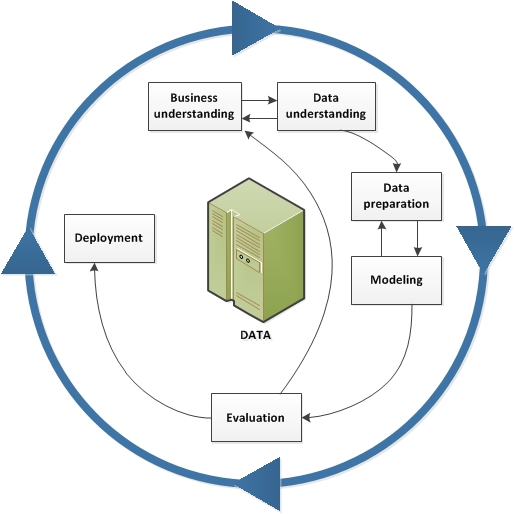
\includegraphics[width=0.8\textwidth]{images/crisp_process.jpg}
%     \caption{The CRISP-DM Process Model (Adapted from IBM SPSS Modeler documentation).}
%     \label{fig:crispdm}
% \end{figure}
% \section{Business Understanding}
% The initial phase of the CRISP-DM framework is centered on defining the project objectives from a business perspective. This end-to-end pipeline is designed to benefit a diverse range of stakeholders who currently face significant challenges in processing spoken Kiswahili. Primary beneficiaries include customer service centers, which can use the system to automatically analyze customer feedback; media and content companies, which can efficiently transcribe and summarize broadcast content; and the education and governance sectors. In education, the system can be used to analyze classroom discourse to improve pedagogical strategies or develop automated tools for language learning by \cite{shearer2000crispdm}. For governance, it provides a crucial tool for summarizing public feedback from community forums, tracking sentiment on policy changes, and gaining real-time insights from citizen feedback hotlines. By providing an automated, low-latency solution, this research will empower these organizations to transform unstructured spoken data into actionable intelligence, thus saving time and resources. Ultimately, this system serves as a foundational tool to democratize access to and analysis of information, directly promoting digital inclusion for the Kiswahili-speaking community.

% The Business Understanding phase serves as the critical conceptual foundation of the project, identifying specific linguistic and technological "pain points" in the processing of Kiswahili digital data and translating them into tangible technical requirements.

% \subsection{Background and Business Objectives}
% Kiswahili stands as a cornerstone of communication for over 200 million individuals across East and Central Africa. Yet, within the global Artificial Intelligence ecosystem, it remains relegated to low-resource status. Historical development in Automatic Speech Recognition (ASR) and Natural Language Processing (NLP) has prioritized Indo-European languages like English and French, creating a digital divide that limits Kiswahili speakers' access to modern education and the digital economy. 

% The central ambition of this research is to dismantle these barriers by engineering an end-to-end pipeline capable of converting raw Kiswahili audio into structured, actionable intelligence. By automating the extraction of insights from unstructured vocal data, this system aims to optimize resource allocation across four transformative sectors. In the realm of \textbf{customer experience}, the pipeline automates feedback analysis to identify service trends without manual intervention. For \textbf{media monitoring}, it enables the efficient indexing and archival of broadcast content for rapid searchability. Within \textbf{educational technology}, the system transcribes classroom discourse to produce automated learning aids and digital notes, while in \textbf{civic governance}, it provides a vital mechanism for summarizing citizen feedback and tracking real-time public sentiment.

% \subsection{Assessment of the Situation}
% A pragmatic deployment of this technology requires addressing several linguistic and operational hurdles. Kiswahili is characterized by intricate morphological structures and diverse regional dialects, often punctuated by Sheng or English code-switching. Beyond linguistics, the operational environment often involves limited computational power and intermittent connectivity in rural or low-income areas. To be viable, the pipeline must be engineered for high computational efficiency, ensuring it can perform on standard hardware with the minimal latency required for near real-time processing in media and service environments.

% \subsection{Data Mining Goals}
% To realize these objectives, the project is structured around four technical milestones. The first milestone focuses on \textbf{transcription accuracy} by fine-tuning Wav2Vec 2.0 architectures to achieve a minimal Word Error Rate (WER) specifically for the Swahili language. Second, we implement \textbf{sentiment extraction} using a DistilBERT-based classifier to categorize transcriptions into positive, negative, or neutral strata for rapid feedback analysis. Third, the project utilizes a Text-to-Text Transfer Transformer (T5) model for \textbf{summarization}, ensuring the core intent of long-form audio is preserved in a concise text format. Finally, \textbf{deployment viability} is achieved by integrating these models into a high-performance FastAPI prototype, demonstrating a seamless, low-latency transition from raw audio input to the final aggregated insights.

% \subsection{Success Criteria}
% Project success is measured by both technical and functional benchmarks. Technically, success is achieved if the pipeline demonstrates accuracy and reliability comparable to established baselines, validated through domain-specific metrics such as WER for transcription, F1-score for sentiment analysis, and ROUGE/BLEU scores for summarization. Functionally, success is defined by the successful integration of these distinct deep learning models into a cohesive, web-based interface that provides a seamless "one-stop" solution for Kiswahili speech analysis. Ultimately, the research aims to provide a foundational tool that fosters digital inclusion and information accessibility for the Kiswahili-speaking community.

% \section{Data Understanding and Collection}
% The Data Understanding phase represents a critical investigative stage within the CRISP-DM framework, involving the acquisition of the primary linguistic corpus and a multi-dimensional analysis of its technical and demographic characteristics. This stage ensures that the empirical foundation is sufficient to support the requirements of the multi-task pipeline.

% \subsection{Data Acquisition and Source}
% The research utilizes the Mozilla Common Voice Corpus 11.0 for Swahili (sw), a premier open-source dataset specifically engineered for the development of Automatic Speech Recognition (ASR) systems. This dataset is compiled through a massive crowdsourcing effort hosted by the Mozilla Foundation, where volunteers contribute recordings of themselves reading prompts. For the purposes of this study, the dataset comprises 14.76 GB of raw Swahili audio data, representing approximately 26,614 individual entries. A defining feature of this source is its built-in peer-validation mechanism; every clip designated as "validated" has successfully passed a review process where multiple contributors voted on the accuracy and clarity of the audio-to-text alignment.

% \subsection{Data Description and Structural Schema}
% A structural audit of the raw data was conducted to map the metadata schema and identify the features available for modeling. The corpus contains seven core columns that provide essential context for each recording. The speaker’s identity is managed via an anonymized unique identifier, while the file system path and the actual audio data stored as a numerical array with an associated sampling rate form the primary input for the ASR module. The target Swahili transcription is stored as a text object. Additionally, peer-validation metrics are tracked through integer counts of "up votes" and "down votes," which indicate the level of community agreement on clip quality. Demographic metadata, such as age and gender, is also present as object data, though these are voluntarily provided by the contributors.

% \subsection{Exploratory Data Analysis and Quality Assessment}
% Following the data collection phase, a comprehensive Exploratory Data Analysis (EDA) was performed to evaluate demographic representation and technical integrity. This audit revealed a significant concentration within the 20--29 age demographic, which accounts for approximately 52\% of the disclosed age data as shownas in Figure~\ref{fig:age_dist}.

% \begin{figure}[h]
% \centering
% 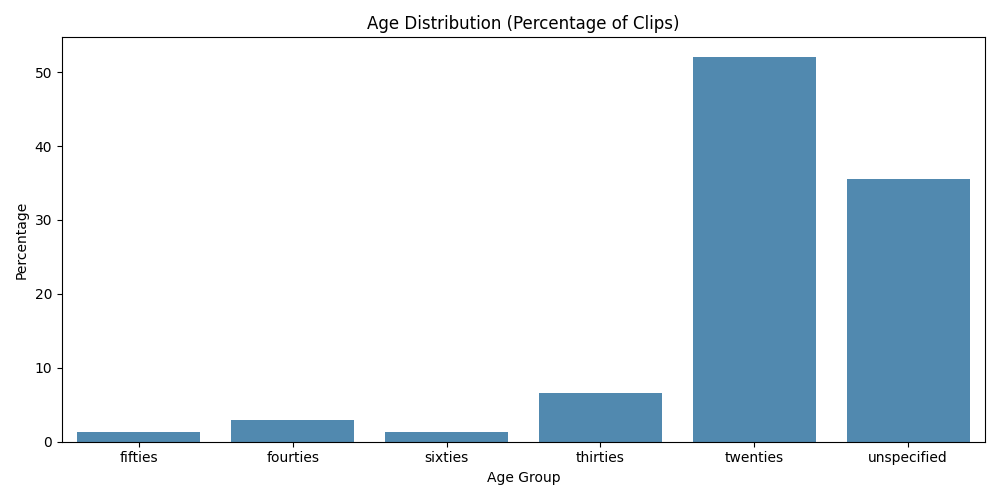
\includegraphics[width=0.8\textwidth]{images/age_distribution_cleaned.pdf}
% \caption{Age distribution of contributors in the Swahili Common Voice corpus}
% \label{fig:age_dist}
% \end{figure}


% In contrast, older age groups, specifically those over 50, are significantly underrepresented, comprising only 2.6\% of the corpus. The gender distribution similarly exhibits a skew, with female speakers representing 36.7\% and male speakers representing 27.7\%, while 35.6\% of the metadata remained undisclosed as revealed in Figure~\ref{fig:gender_dist}. 

% \begin{figure}[h]
% \centering
% 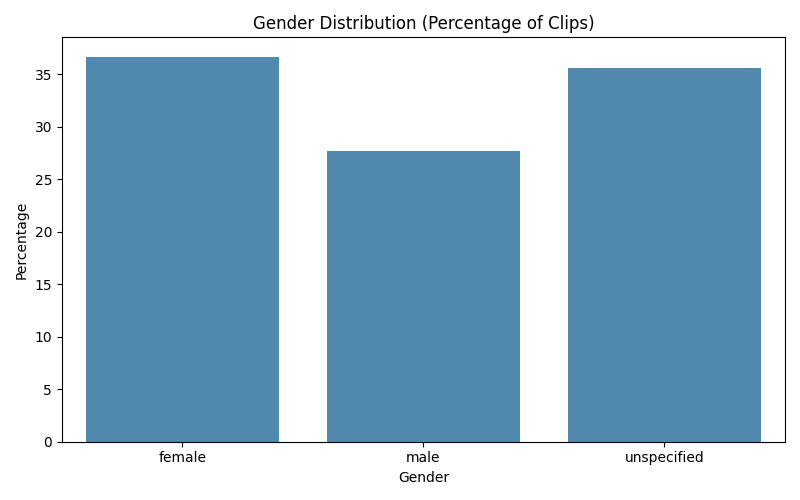
\includegraphics[width=0.8\textwidth]{images/gender_distribution_cleaned.pdf}
% \caption{Gender distribution of contributors including undisclosed metadata}
% \label{fig:gender_dist}
% \end{figure}

% To mitigate this missingness and maintain data integrity during model training, a neutral placeholder strategy was adopted to categorize unspecified entries.

% \noindent The technical quality analysis was further informed by contributor and validation metrics. The dataset includes contributions from approximately 76 unique speakers. The calculated validation ratio, representing the proportion of down-votes to total votes, stands at 0.1287. This indicates that roughly 12.8\% of the data was flagged for potential quality issues by the community, providing a clear justification for the rigorous cleaning protocols implemented in the subsequent data preparation phase. A bivariate correlation analysis between transcript length and rejection rates (Pearson $r = 0.004$) revealed no meaningful relationship between the length of a sentence and the likelihood of it being down-voted, as illustrated in Figure~\ref{fig:vote_length}. 

% \begin{figure}[h]
% \centering
% 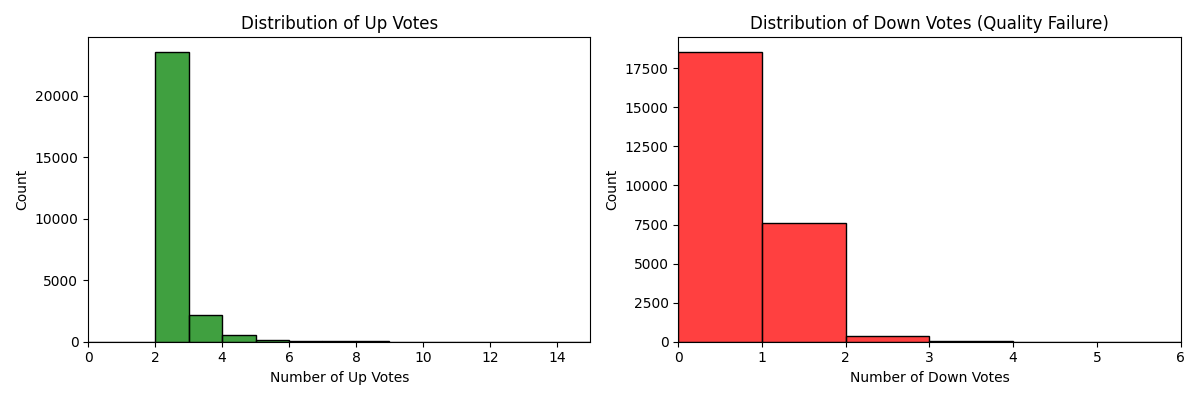
\includegraphics[width=0.85\textwidth]{images/votes_distribution.pdf}
% \caption{Relationship between sentence length and down-vote ratio}
% \label{fig:vote_length}
% \end{figure}

% This suggests that validation failures are primarily driven by acoustic factors, such as background noise or articulation, rather than the linguistic complexity of the prompts.

% \noindent The linguistic characterization of the corpus revealed a median sentence length of 9.0 words and a mean word length of 5.46 characters. N-gram frequency analysis in Figure~\ref{fig:bigrams} highlighted the phrasal backbone of the dataset, with unigrams such as "ya", "na", and "wa" appearing with the highest frequency. Bigram analysis identified critical phrasal patterns such as "elfu moja", "baada ya", and "moja mia", which are essential for maintaining semantic coherence during transcription. 

% \begin{figure}[H]
% \centering
% 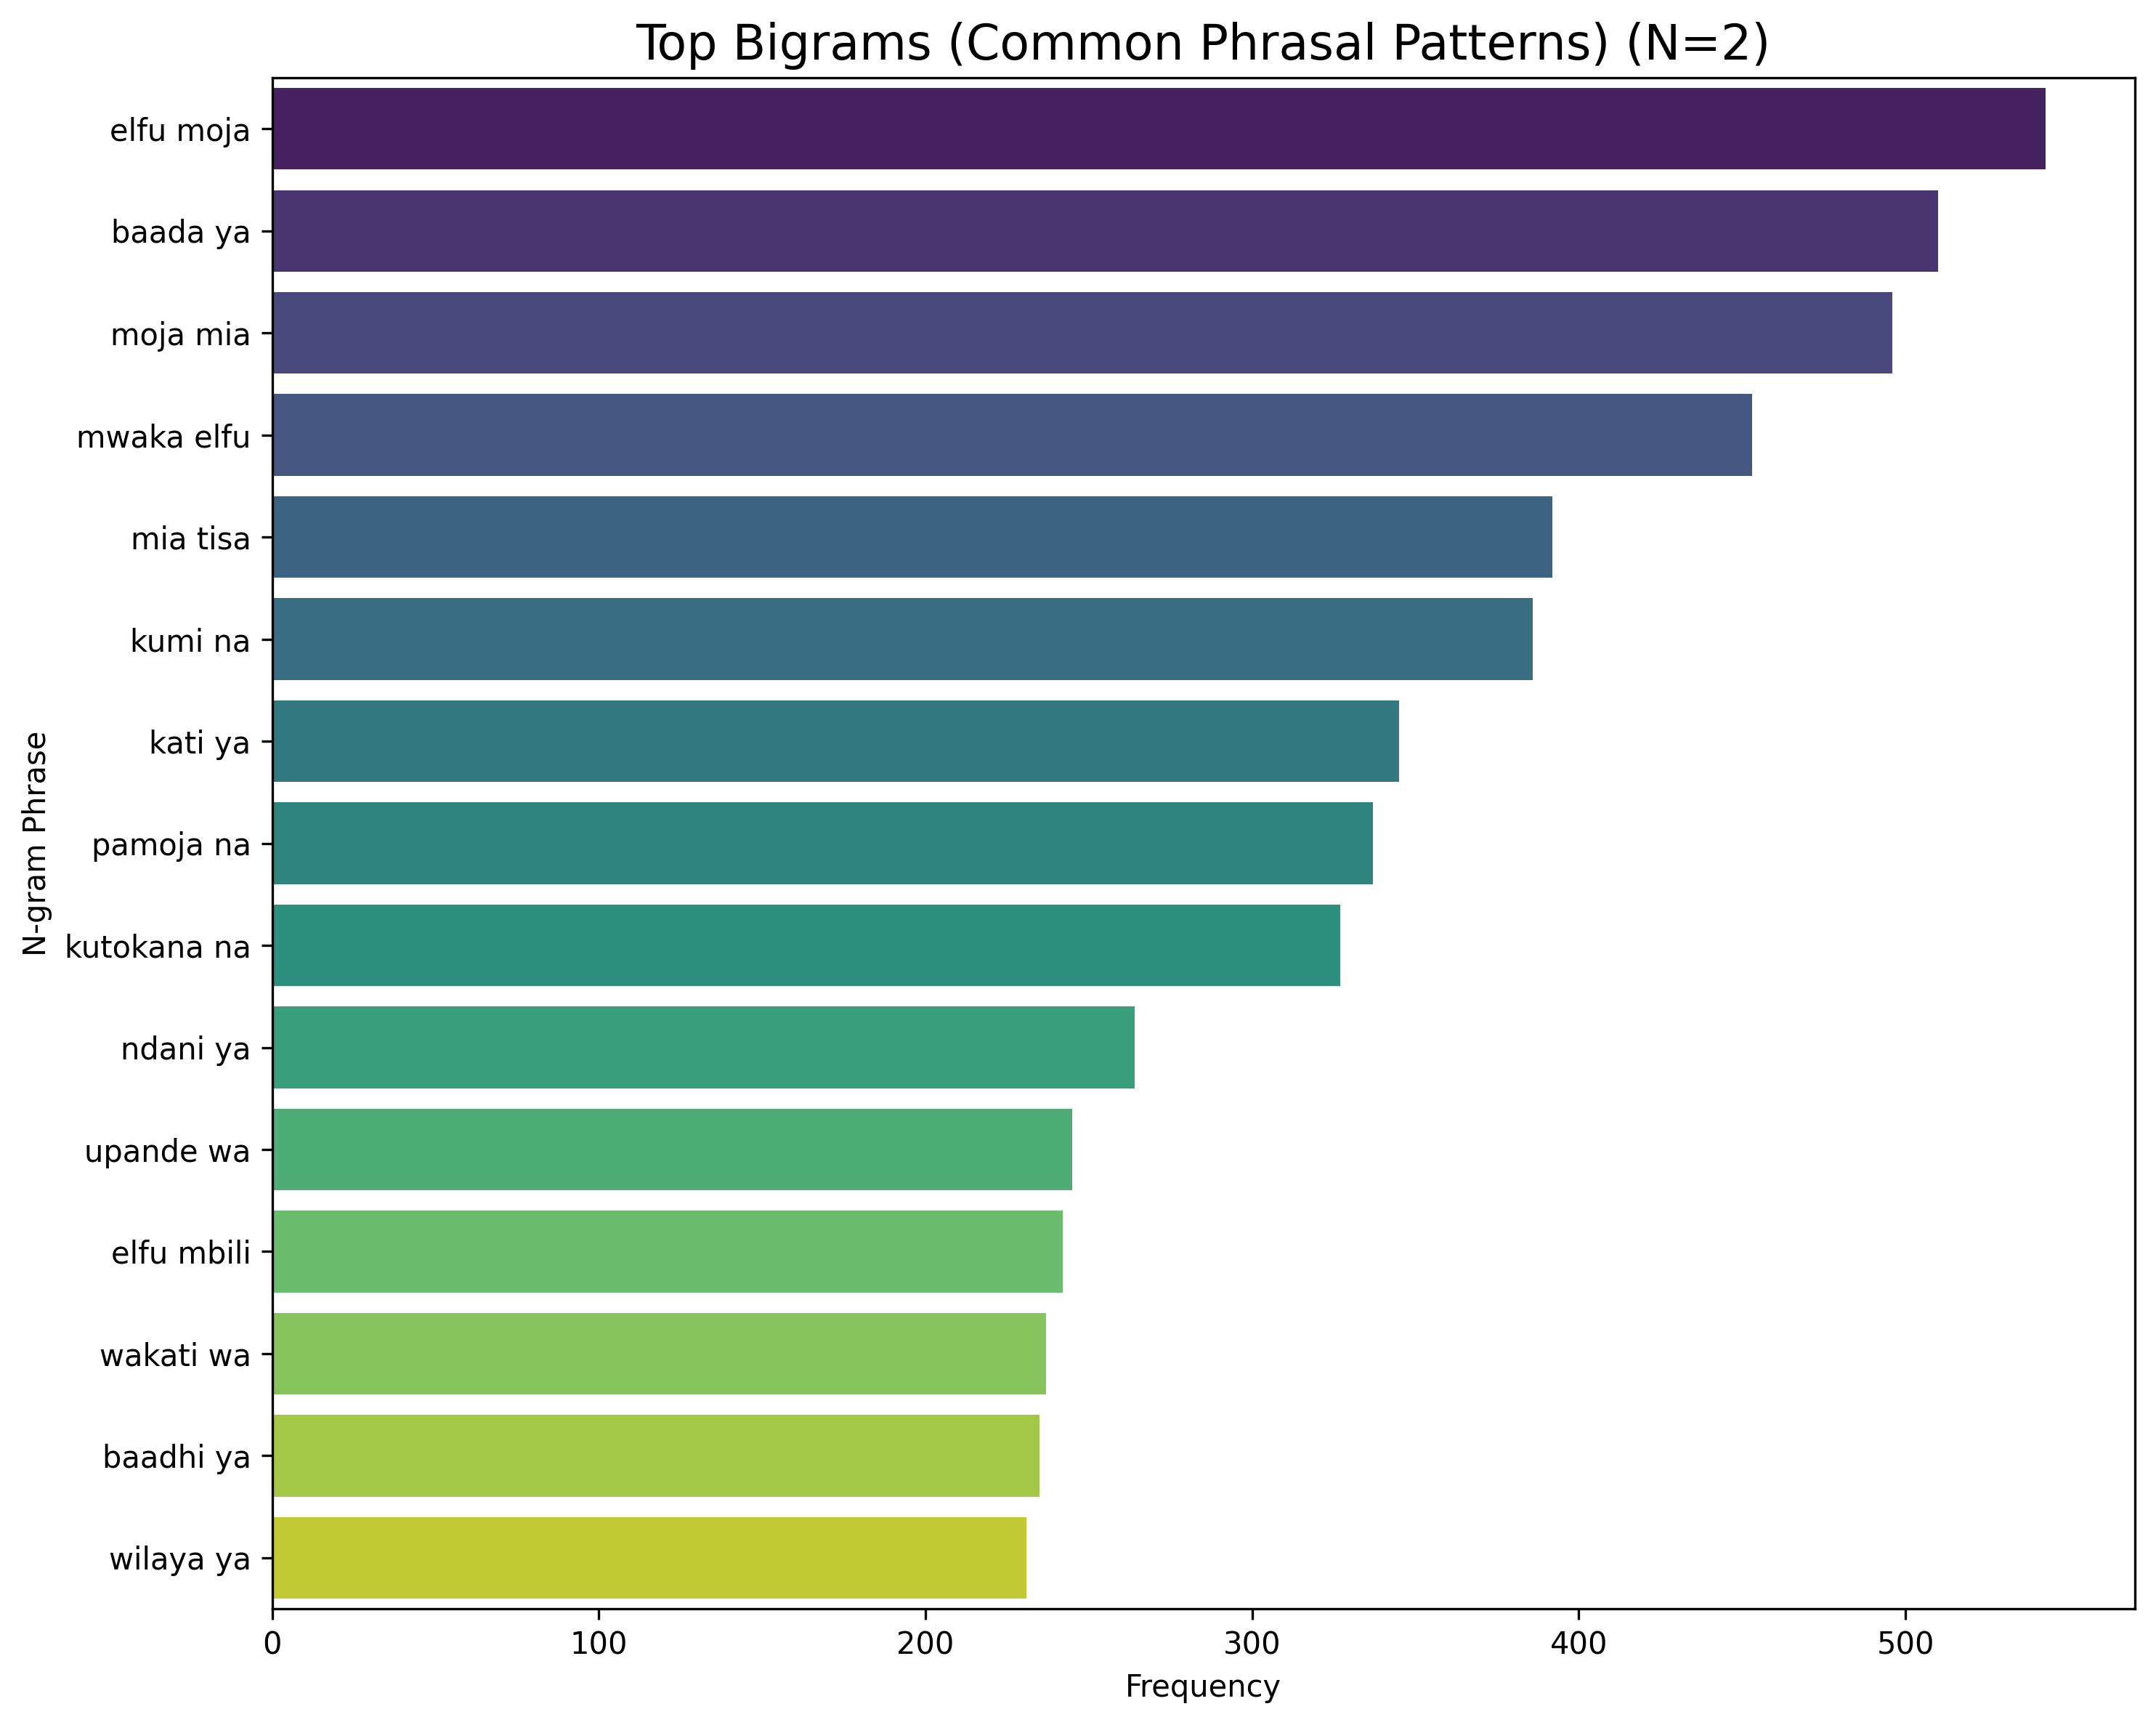
\includegraphics[width=0.6\textwidth]{images/top_bigrams_(common_phrasal_patterns).pdf}
% \caption{Most frequent Swahili bigrams illustrating phrasal structure}
% \label{fig:bigrams}
% \end{figure}


% The final assessment for completeness highlighted that columns such as "Accent" and "Segment" were entirely missing and irrecoverable. Linguistically, an audit of target sentences confirmed the presence of the phonetic apostrophe and loanword characters such as 'q' and 'x', informing the requirement for a 58-token vocabulary to ensure the ASR model captures the full semantic breadth of Kiswahili.

% \subsection{Text and Unstructured Data Analytics}
% This phase involves analyzing the thematic content of the corpus to justify the linguistic preprocessing required for high-accuracy NLP tasks. A critical step included the development of a custom library of Swahili stop-words, categorized into 17 linguistic groups such as \textit{Viashiria} (demonstratives), \textit{Viwakilishi} (pronouns), and \textit{Vitenzi Msaada} (auxiliary verbs). Comparing word clouds before and after stop-word removal visually demonstrates the high density of "noise" in low-resource language data, as shown in Figure~\ref{fig:wordcloud}. This thematic extraction is vital for ensuring that subsequent components, such as Sentiment Analysis and Summarization, focus on sentiment-bearing keywords and core intent rather than functional particles.

% \begin{figure}[h]
% \centering
% 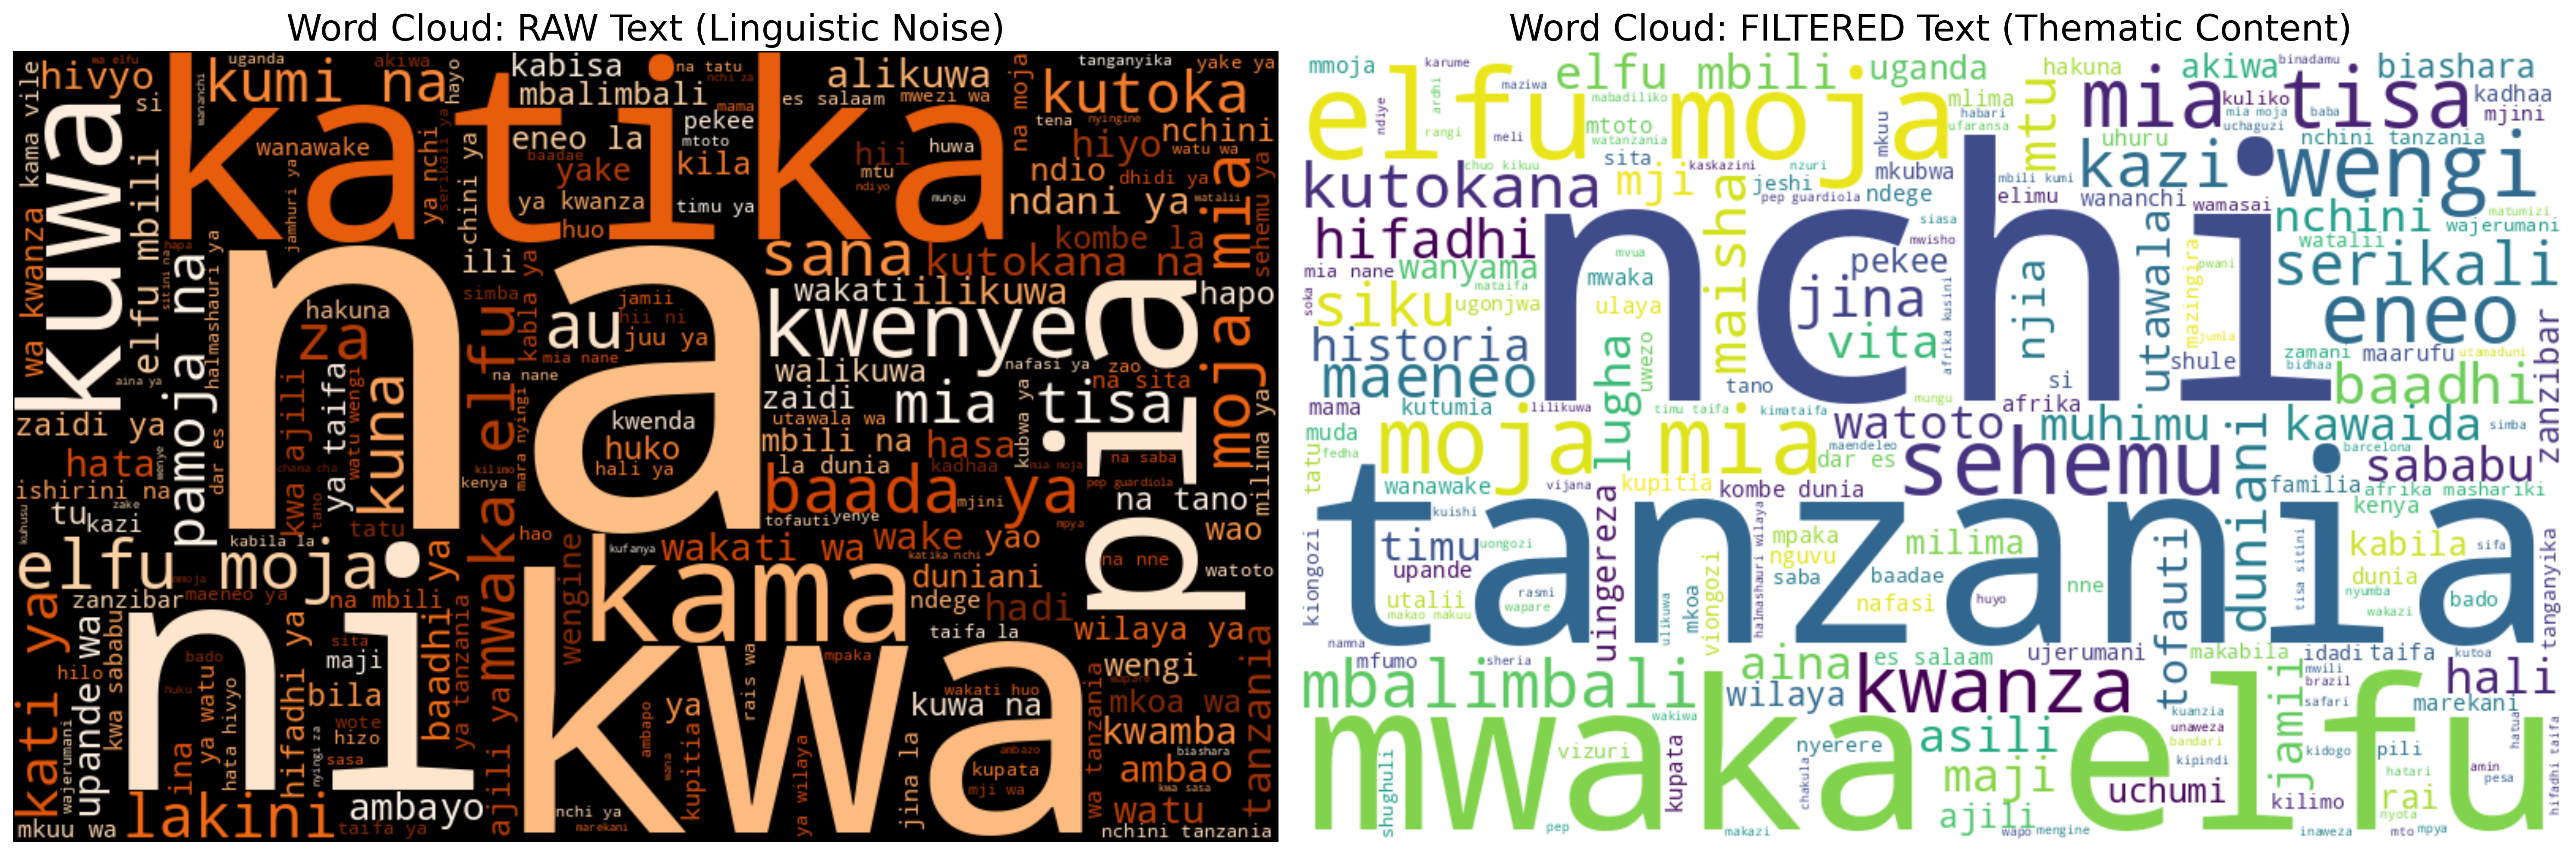
\includegraphics[width=\textwidth]{images/wordcloud_comparison.png}
% \caption{Word cloud comparison before and after Swahili stop-word removal}
% \label{fig:wordcloud}
% \end{figure}


% \noindent\textbf{Exploratory Sentiment Characterization.}

% As part of the unstructured text analytics, an exploratory sentiment inference was conducted on the transcribed Kiswahili sentences to assess the affective distribution of the corpus. This analysis employed a pretrained multilingual transformer-based sentiment model applied directly to the text. The purpose of this step was not to construct a supervised sentiment classifier, but rather to characterize the emotional properties of the dataset and evaluate its suitability for downstream semantic analysis.

% The inferred sentiment distribution revealed a strong dominance of neutral classifications, with positive and negative sentiments occurring only marginally. This outcome aligns with the functional and instructional design of the Common Voice prompts, which are primarily declarative and phonetically motivated rather than emotionally expressive. Examination of model confidence scores further indicated weak class separation, suggesting that affective cues within the corpus are sparse and contextually ambiguous.

% Given the absence of ground-truth sentiment annotations and the low emotional variance observed, conventional supervised evaluation metrics such as precision, recall, and F1-score were deemed methodologically inappropriate. Consequently, the results are reported descriptively through label distributions, confidence scores, and representative example predictions. These findings confirm that sentiment analysis, while feasible as an auxiliary post-transcription task, does not constitute a reliable predictive objective for this dataset.

% Importantly, the observed neutrality bias serves as an empirical validation of the corpus design and supports the exclusion of sentiment features from the core ASR training pipeline, while still permitting their optional inclusion for exploratory analysis and metadata enrichment.


% \section{Data Cleaning and Preprocessing}
% To ensure the accuracy, reliability, and computational efficiency of the subsequent machine learning models, the raw Kiswahili dataset underwent a comprehensive cleaning and preprocessing pipeline. This phase was designed to mitigate the inherent "noise" of crowdsourced data, reduce irrelevant computational overhead, and standardize both audio and textual inputs to facilitate effective model training. The pipeline comprised several specialized stages: audio silence trimming, spectral noise reduction, text normalization, and robust metadata validation.

% \subsection{Silence Trimming}
% The initial stage of audio preprocessing focused on the removal of non-informative silent segments from the temporal boundaries of each recording. Utilizing the \texttt{librosa.effects.trim()} function, the system automatically identified and removed segments where the decibel level fell below a predefined threshold as illustrated in Figure~\ref{fig:silence_trim}. 

% The retention of leading or trailing silence offers no instructional value for Automatic Speech Recognition (ASR) training. These segments artificially inflate the duration of audio clips, resulting in increased processing latency and higher computational costs during the feature extraction and modeling phases. 

% \begin{figure}[h]
% \centering
% 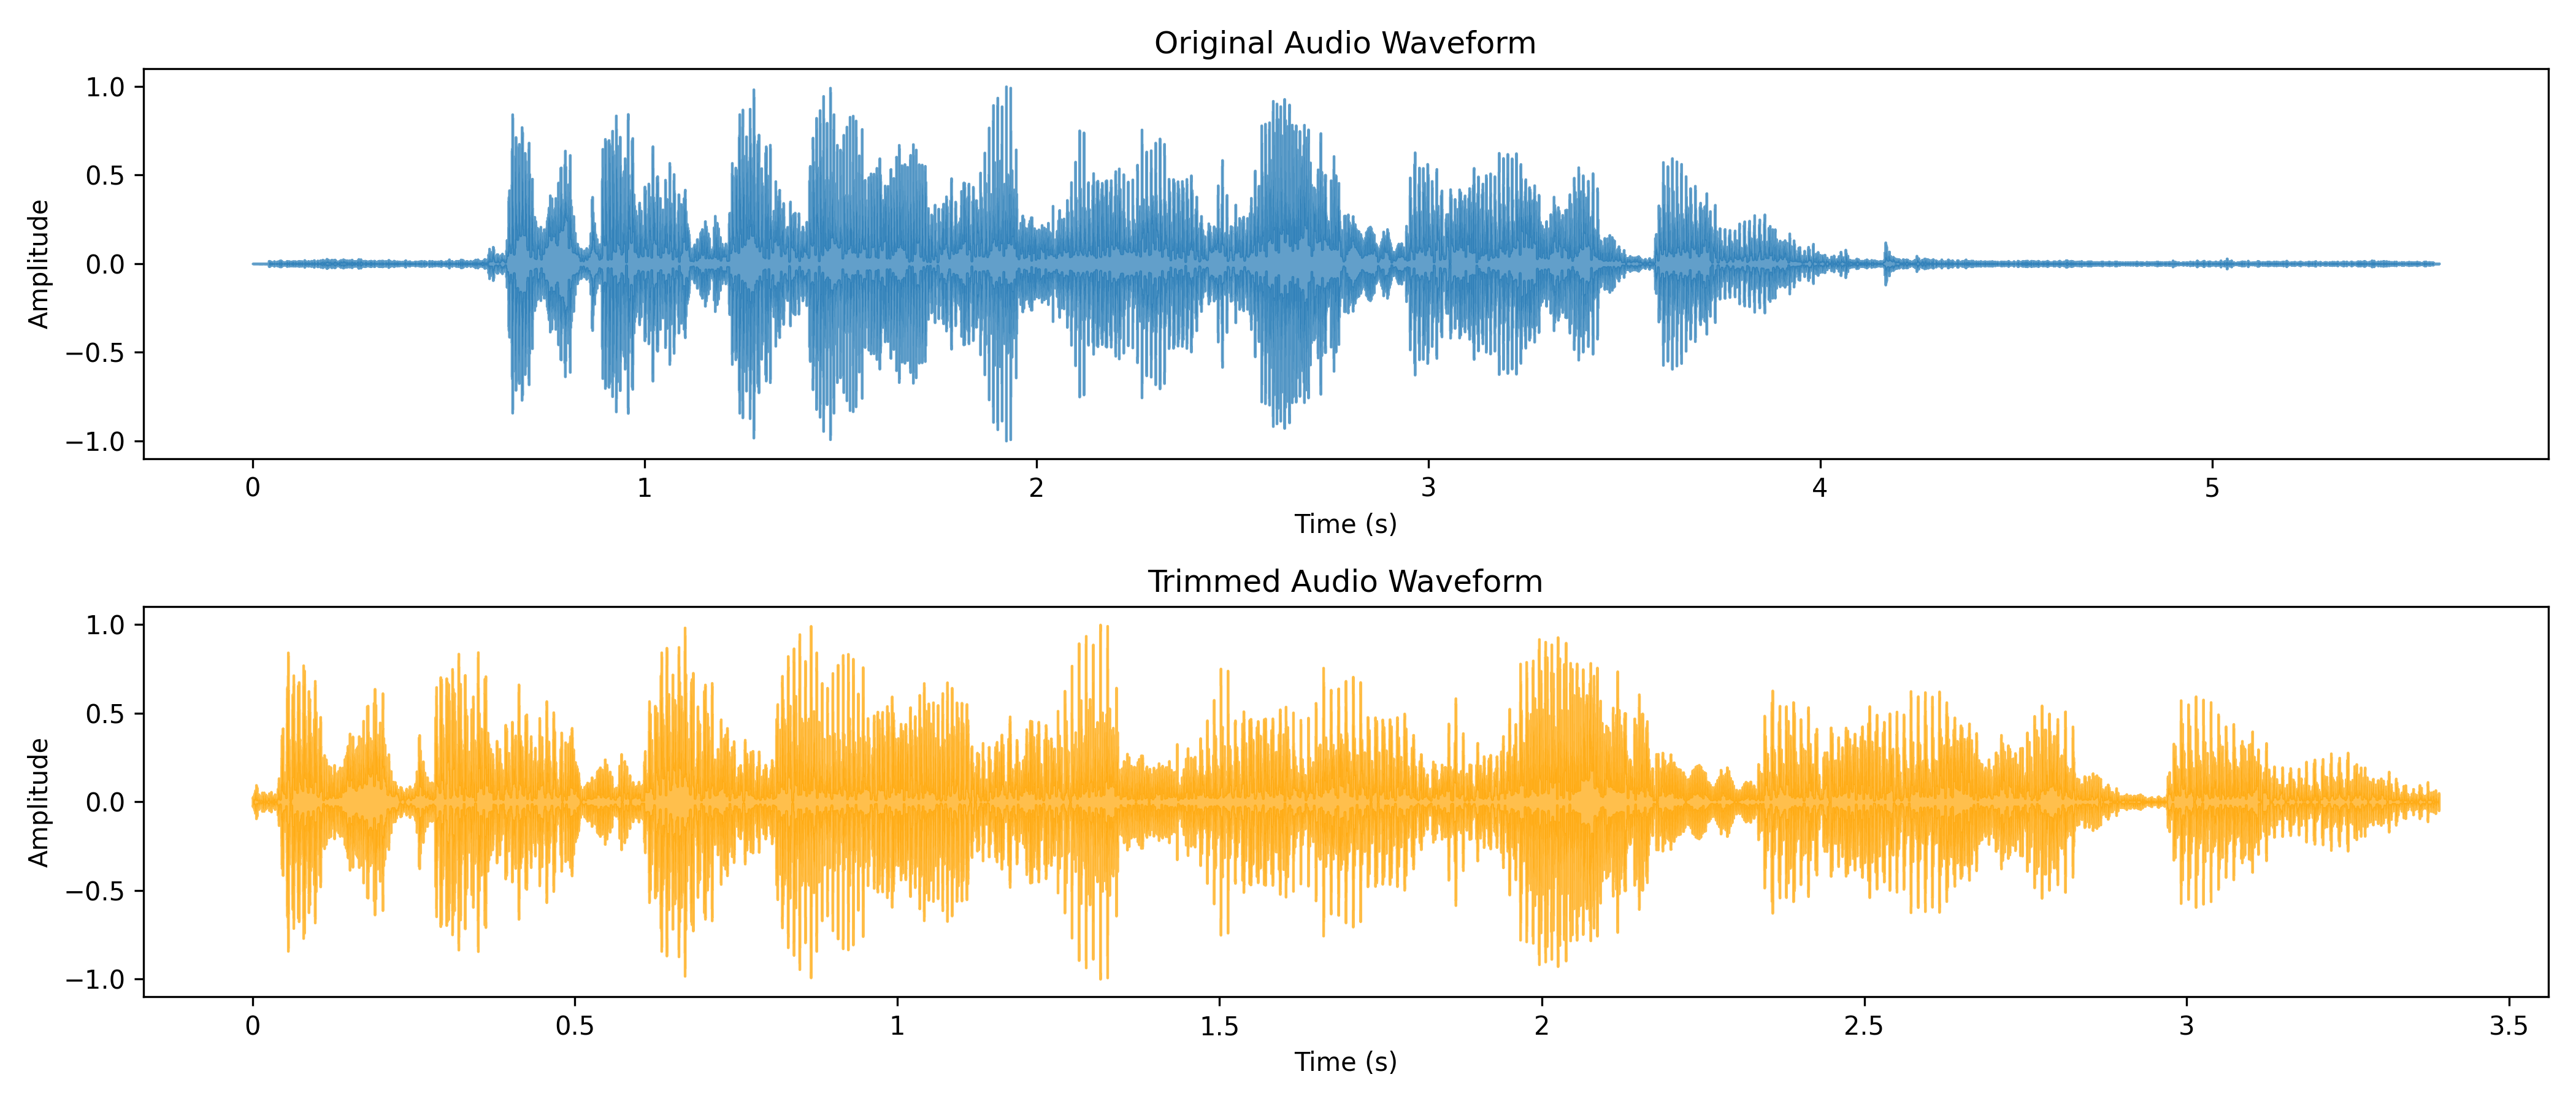
\includegraphics[width=\textwidth]{images/silence_trimming_comparison.pdf}
% \caption{Waveform comparison before and after silence trimming}
% \label{fig:silence_trim}
% \end{figure}


% Furthermore, eliminating these segments prevents the model from inadvertently learning patterns unrelated to speech, thereby reducing the risk of overfitting and enhancing the model's ability to generalize to natural, continuous speech.

% Mathematically, the trimming process is defined by the following energy-based selection:
% \begin{equation}
% \text{Trimmed Audio} = \{ \text{Audio}[t] \mid \text{Energy}(\text{Audio}[t]) > \tau \}
% \end{equation}
% Where:
% \begin{itemize}
%     \item $\text{Audio}[t]$ represents the discrete audio signal at time $t$.
%     \item $\text{Energy}(\text{Audio}[t]) = |\text{Audio}[t]|^2$ represents the instantaneous energy of the signal.
%     \item $\tau$ is the predefined energy threshold distinguishing active speech from background silence.
% \end{itemize}

% \subsection{Noise Reduction via Spectral Gating}
% To enhance the clarity of the speech signal, a spectral gating algorithm was implemented using the \texttt{pydub} library. Background noise, such as environmental hums or static, can significantly degrade ASR performance by creating spectral distortions that confuse the encoder during training. 

% The algorithm functions by first calculating a ``noise floor'' based on the initial $1/10^{\text{th}}$ of the audio signal, assuming this segment contains only background ambient noise. Mathematically, the noise floor is derived as:
% \begin{equation}
% \text{Noise Floor} = \frac{1}{n} \sum_{i=1}^{n} |S(f, t)_i|
% \end{equation}

% where $n$ represents the number of samples in the initial segment and $|S(f, t)_i|$ is the absolute value of the $i$-th component in the spectrogram. The noise threshold is subsequently set as twice the noise floor ($\tau = 2 \times \text{Noise Floor}$). The cleaning process follows a gating logic:
% \begin{equation}
% S_{\text{clean}}(f, t) = 
% \begin{cases} 
% S(f, t) & \text{if } |S(f, t)| > \tau \\
% 0 & \text{if } |S(f, t)| \leq \tau 
% \end{cases}
% \end{equation}

% A visual comparison of the spectrograms before and after noise suppression illustrates the effectiveness of this approach, as shown in Figure~\ref{fig:noise_reduction}.

% \begin{figure}[H]
% \centering
% 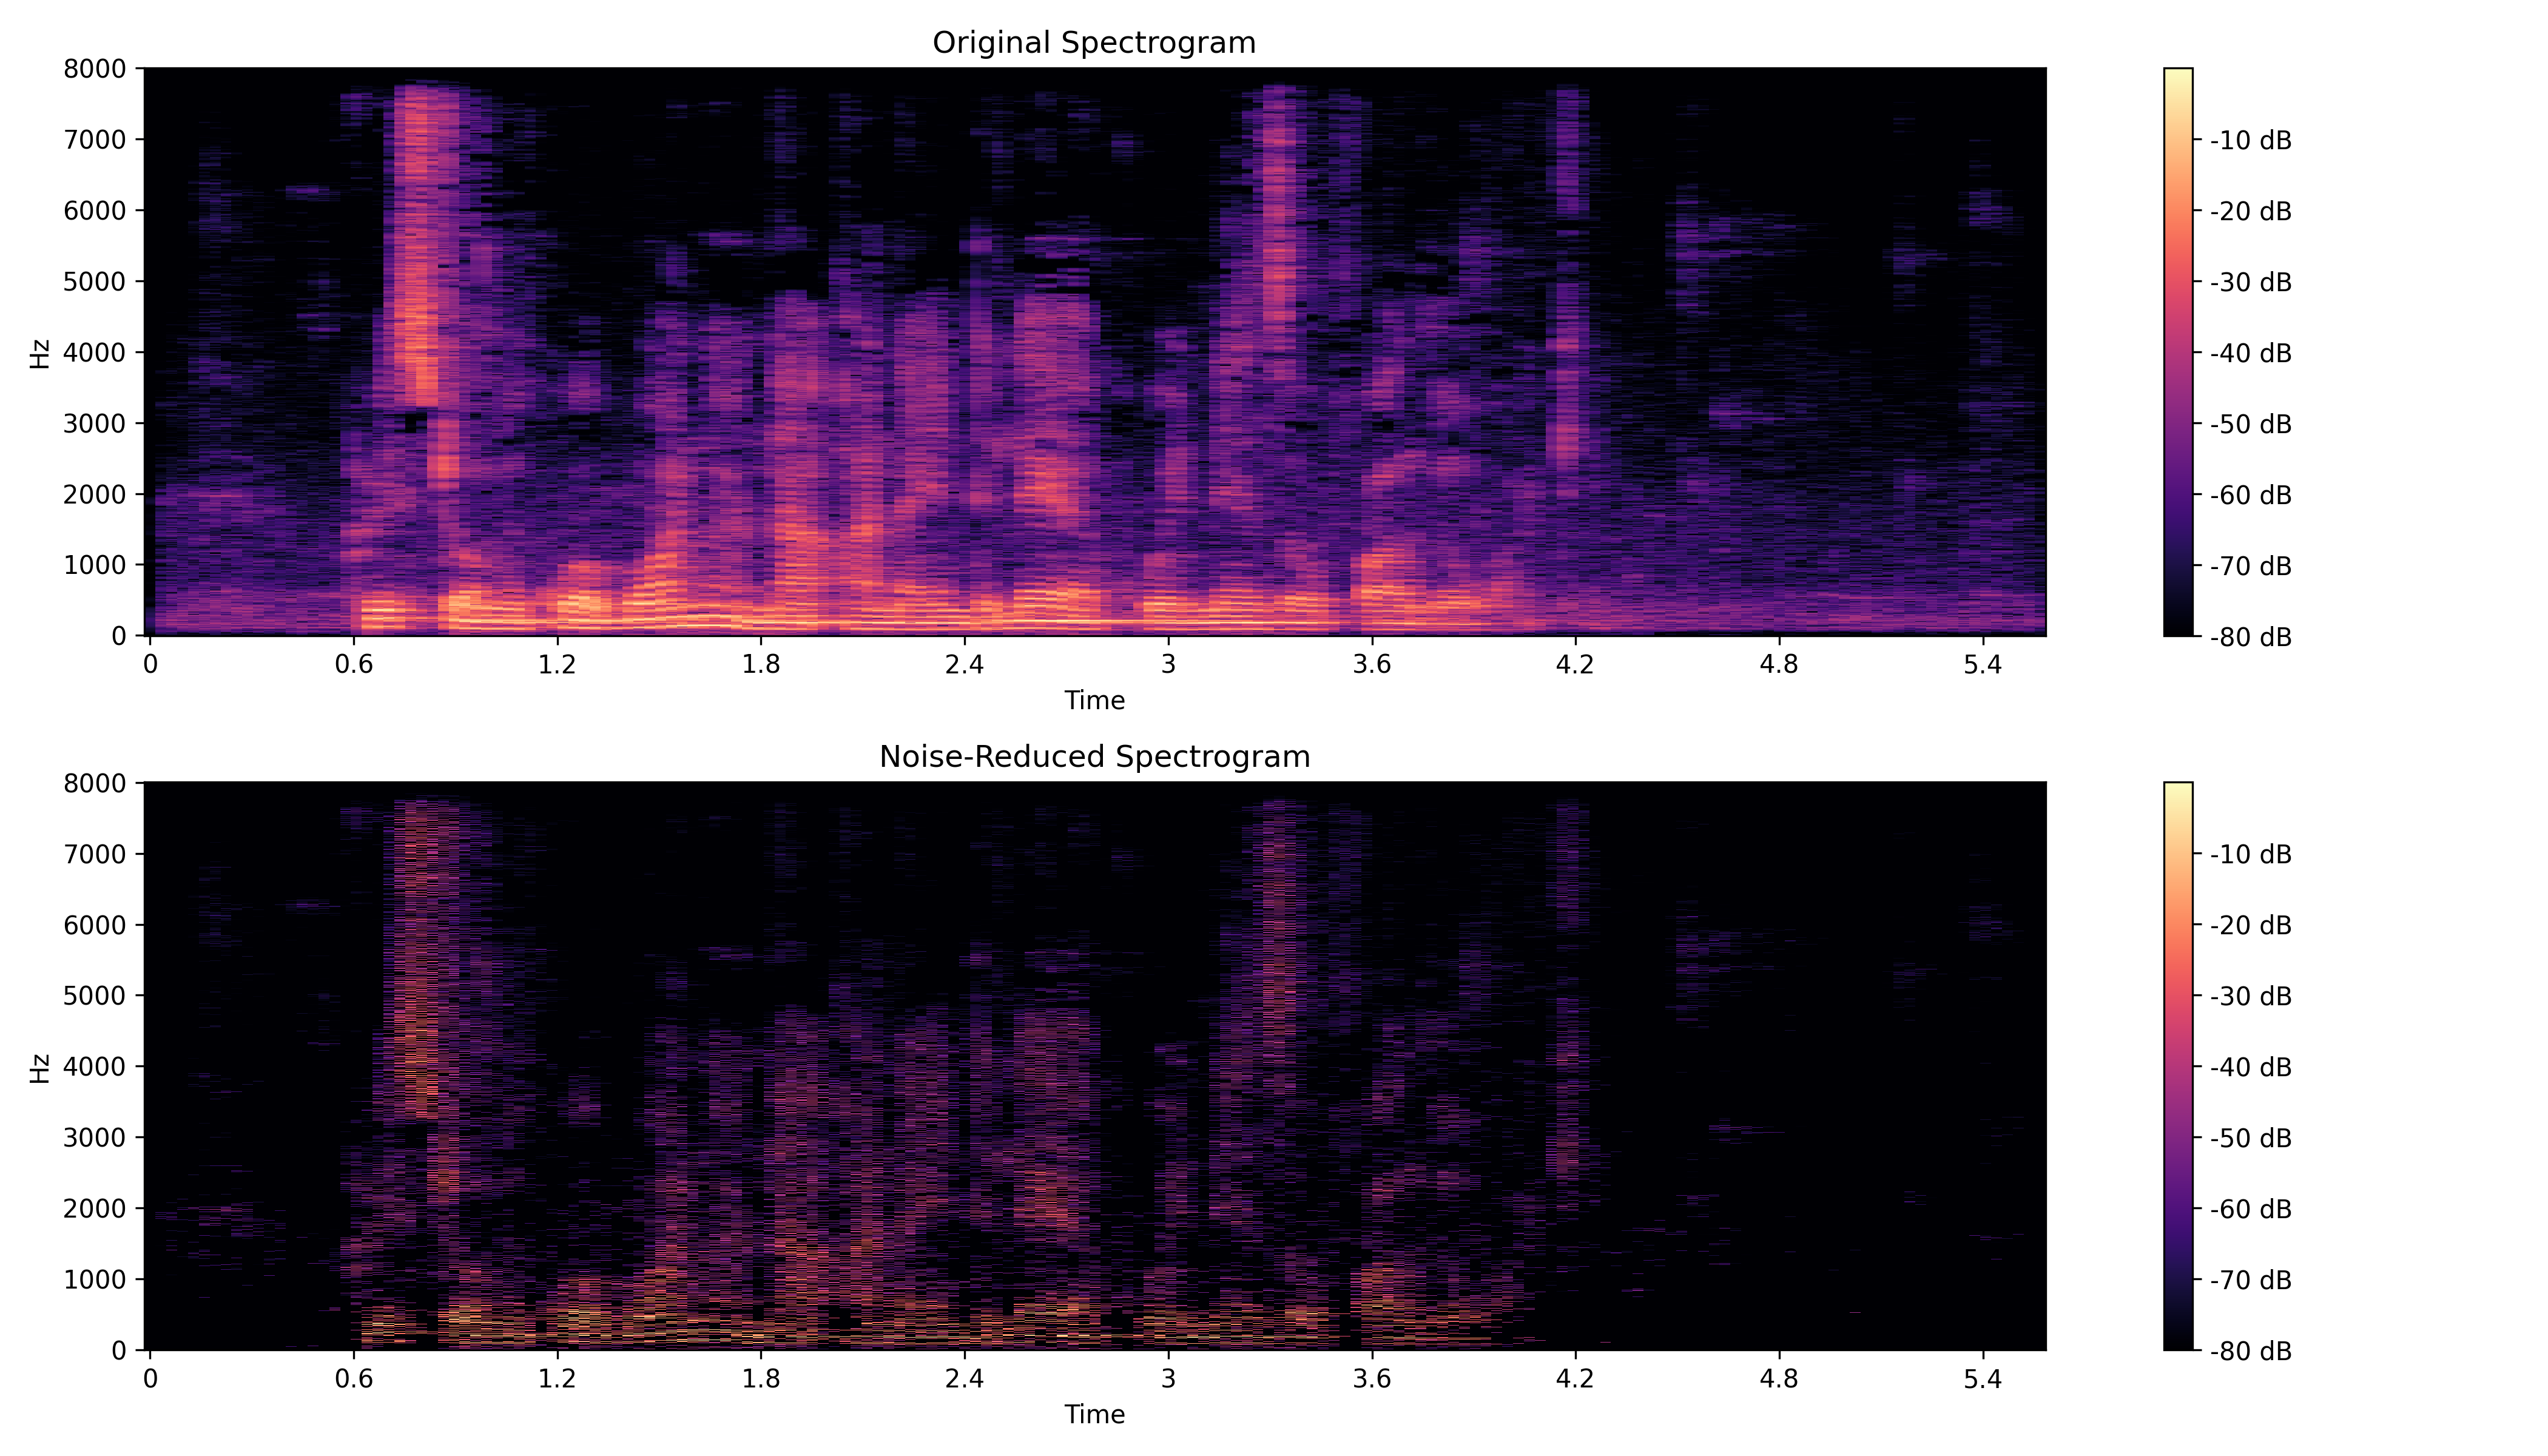
\includegraphics[width=\textwidth]{images/noise_reduction_spectrogram.pdf}
% \caption{Spectrogram comparison before and after spectral noise reduction}
% \label{fig:noise_reduction}
% \end{figure}

% This ensures that only frequency components with sufficient energy to likely represent speech are preserved, resulting in a cleaner signal that improves transcription accuracy across diverse acoustic environments.


% \subsection{Text Normalization}
% Text normalization was performed to standardize the linguistic targets and reduce data complexity. This step ensured the model focused on semantic patterns rather than orthographic variations. The normalization process included converting all text to lowercase and stripping non-essential punctuation. Critically, for the Kiswahili context, the phonetic apostrophe ($'$) was preserved, as it holds semantic significance. Additionally, a custom library of stop-words was utilized to prune functional particles during the sentiment analysis and summarization preparation, allowing the models to concentrate on high-entropy keywords.

% \subsection{Handling Missing Values and Metadata Validation}
% Incomplete metadata poses a risk of introducing systematic bias, particularly when utilizing demographic features like age or gender for performance auditing. Rather than discarding records with missing values which would result in a loss of valuable acoustic data, this research utilized a neutral placeholder strategy. Missing categorical entries were imputed with the string "unknown" or "unspecified." This approach maintains the integrity of the total dataset, ensures uniform representation across all data points, and prevents the unjustifiable exclusion of contributors from the training set, thereby supporting a more robust and inclusive final model.

% \subsection{Acoustic Feature Extraction}
% Following cleaning, the audio was transformed into structured representations. Mel-Frequency Cepstral Coefficients (MFCCs) were extracted to summarize the spectral envelope most relevant to human speech perception. Additionally, Mel spectrograms were generated using a Short-Time Fourier Transform (STFT) to map the signal into a two-dimensional time-frequency representation. These features provide a critical balance between dimensionality reduction and the preservation of phonetic information required for high-accuracy ASR.

% \section{Machine Learning Modeling}

% The core architecture employs a suite of Transformer-based models optimized for distinct linguistic tasks. In the current study, only the ASR module is fine-tuned on the Swahili dataset, while sentiment analysis and summarization leverage pre-trained multilingual models for inference.

% \subsection{Speech Recognition: Wav2Vec 2.0}
% The primary engine for Automatic Speech Recognition (ASR) in this research is the \textit{"eddiegulay/wav2vec2-large-xlsr-mvc-swahili"} model. This architecture represents a sophisticated application of the Wav2Vec 2.0 framework, specifically fine-tuned for the phonetic and morphological nuances of the Swahili language. The model is built upon the Cross-lingual Speech Representations (XLSR) approach, which leverages large-scale pre-training on thousands of hours of multilingual speech to learn a universal acoustic subspace.

% The learning objective of this model is centered on a self-supervised contrastive task. It is optimized by minimizing a contrastive loss function ($\mathcal{L}_{\text{ASR}}$), which forces the model to distinguish a true quantized latent speech representation from a set of negative ``distractor'' samples within a shared embedding space. This is mathematically expressed as:

% \begin{equation}
%     \mathcal{L}_{\text{ASR}} \propto - \log \frac{e^{\text{sim}(\mathbf{z}_v, \mathbf{c}_v) / \kappa}}{\sum_{\tilde{\mathbf{z}} \in \mathbb{Z}} e^{\text{sim}(\tilde{\mathbf{z}}, \mathbf{c}_v) / \kappa}}
% \end{equation}

% where $\mathbf{z}_v$ denotes the predicted quantized latent representation at time $v$, $\mathbf{c}_v$ represents the true context representation generated by the Transformer layers, $\text{sim}$ computes the cosine similarity between these vectors, $\kappa$ is a constant temperature scaling factor, and $\mathbb{Z}$ represents the union of the true target and $K$ distractor representations.

% The implementation of this specific model provides several critical advantages for Swahili speech analysis:
% \begin{itemize}
%     \item \textbf{Cross-Lingual Transfer Learning:} As Swahili is a low-resource language regarding high-fidelity labeled acoustic data, the XLSR-based variant is essential. It enables the system to benefit from acoustic patterns learned from high-resource languages, significantly improving the recognition of Swahili phonemes even with limited native training data.
    
%     \item \textbf{Raw Waveform Feature Extraction:} Unlike traditional ASR systems that rely on manually engineered features like Mel-frequency cepstral coefficients (MFCCs), Wav2Vec 2.0 utilizes a multi-layer convolutional neural network (CNN) as a feature encoder. This allows the model to process raw audio waveforms directly, capturing fine-grained temporal and spectral details that are typically lost in standard spectrogram conversions.
    
%     \item \textbf{Contextual Modeling via Transformers:} Following feature extraction, a deep Transformer architecture is utilized to capture long-range dependencies in the speech signal. This is vital for Swahili, where word meaning is heavily dependent on agglutinative structures such as prefixes and suffixes.
    
%     \item \textbf{Connectionist Temporal Classification (CTC):} The model employs a CTC decoding head to map continuous audio signals to discrete text characters. This facilitates an ``end-to-end'' training approach that does not require the audio to be pre-aligned with the transcript, streamlining the inference pipeline for real-world Swahili dialogue.
% \end{itemize}

% This strategic choice of the Wav2Vec 2.0 architecture ensures that the system achieves high transcription accuracy even in the presence of varying accents and background noise, ultimately resulting in a robust foundation for downstream exploratory semantic analysis and abstractive summarization.

% \subsection{Sentiment Analysis: DistilBERT(Pre-trained)}
% For exploratory semantic characterization of the transcribed output, the system applies a pretrained multilingual sentiment inference model, specifically \textit{"lxyuan/distilbert-base-multilingual-cased-sentiments-student"}. 

% Unlike the ASR components, this module is not trained or fine-tuned within this research and does not rely on ground-truth sentiment annotations. Instead, it operates as a zero-shot, model-inferred analytical layer used to assess whether affective signals are meaningfully present in the automatically generated Swahili transcripts.

% While the underlying model was originally optimized using a Cross-Entropy Loss function ($\mathcal{L}_{\text{Sentiment}}$)  during its pretraining phase, no supervised loss optimization was performed in this study. The model was used strictly in inference mode to generate probabilistic sentiment distributions over predefined classes, which were subsequently analyzed descriptively rather than evaluated against labeled ground truth.

% \begin{equation}
%     \mathcal{L}_{\text{Sentiment}} = - \frac{1}{N} \sum_{i=1}^{N} \sum_{c=1}^{C} y_{i,c} \log(\hat{y}_{i,c})
% \end{equation}

% where $N$ denotes the total number of samples, $C$ represents the number of sentiment classes, $y_{i,c}$ is a binary indicator (0 or 1) if class label $c$ is the correct classification for observation $i$, and $\hat{y}_{i,c}$ is the predicted probability of observation $i$ belonging to class $c$.

% The selection of this "student" distilled model over larger, more traditional architectures such as BERT-Large or RoBERTa is justified by several critical technical factors essential for a real-time Swahili ASR pipeline:

% \begin{itemize}
%     \item \textbf{Knowledge Distillation Efficiency:} This model utilizes a teacher-student framework where a smaller model (the student) is trained to reproduce the behavior of a larger, more complex model (the teacher). This results in a model that retains approximately 97\% of the teacher's performance while being 40\% smaller and 60\% faster, making it ideal for deployment on hardware with limited resources, such as CPUs.
    
%     \item \textbf{Multilingual Generalization:} Unlike English-centric sentiment models, the cased multilingual nature of this model allows it to handle the nuances of Swahili text. It effectively processes capital letters and regional phonetic markers which are crucial for maintaining semantic context in low-resource linguistic environments.
    
%     \item \textbf{Inference Latency Reduction:} In a production environment using FastAPI, the bottleneck is often the acoustic model. By utilizing a "student" DistilBERT, we minimize the overhead of the sentiment head, allowing the system to process transcripts nearly instantaneously without increasing the total end-to-end response time.
    
%     \item \textbf{Robustness to Noisy Transcripts:} Student models often exhibit better generalization when faced with slightly imperfect transcripts, such as those generated in ASR tasks, as they focus on the most significant semantic features learned from the teacher model rather than overfitting to specific training noise.

%     \item \textbf{Exploratory Role in the Pipeline:} Sentiment inference was treated as a diagnostic and descriptive component rather than a predictive objective. Observed class distributions and confidence scores were used to assess corpus characteristics and to inform downstream analytical decisions, not to optimize or validate model performance.
% \end{itemize}

% This strategic choice ensures that the final system provides high-fidelity sentiment classification while maintaining the high performance required for real-world application.

% \subsection{Text Summarization: mT5-small (Pre-trained)}
% The final stage of the linguistic processing pipeline involves abstractive summarization using the \textit{google/mt5-small} model. This architecture is based on the Text-to-Text Transfer Transformer (T5) framework, which conceptualizes every Natural Language Processing (NLP) task, including summarization as a sequence-to-sequence mapping problem. 

% The model was not fine-tuned on the Swahili dataset due to the failure of training attempts on noisy ASR transcripts. Instead, zero-shot summarization is used for exploratory text summarization of the transcriptions. generating the correct target summary tokens ($\mathcal{L}_{\text{T5}}$) in the input transcription:

% \begin{equation}
%     \mathcal{L}_{\text{T5}} = - \sum_{t} \log P(\mathbf{y}_t^* \mid \mathbf{y}_{<t}^*, \mathbf{x}; \theta)
% \end{equation}

% In this equation, $\mathbf{y}_t^*$ represents the ground-truth target token at time step $t$, $\mathbf{y}_{<t}^*$ denotes the sequence of tokens generated in previous steps, $\mathbf{x}$ is the input Swahili transcription, and $\theta$ represents the trainable model parameters.

% The selection of the \textit{mT5-small} variant for this research is justified by several comprehensive technical considerations:

% \begin{itemize}
%     \item \textbf{Massively Multilingual Pre-training:} Unlike the standard T5 model, which is primarily trained on English datasets (C4), the mT5 model is pre-trained on the mC4 corpus, which encompasses over 101 languages, including Swahili. This cross-lingual pre-training allows the model to leverage "transfer learning" from high-resource languages to effectively understand the syntax and semantics of Swahili, despite it being a lower-resource language in the digital domain.
    
%     \item \textbf{Abstractive Summarization Capability:} By treating summarization as conditional text generation, the model can produce novel, grammatically correct Swahili sentences that capture the core meaning of the transcript, rather than relying solely on extractive methods.
    
%     \item \textbf{Computational Efficiency and Deployment:} The "small" variant of mT5 was specifically chosen to balance linguistic capability with deployment feasibility. With approximately 300 million parameters, the model is significantly more lightweight than its \texttt{base} or \texttt{large} counterparts. This reduction in parameter count is critical for minimizing the memory footprint and inference latency when hosted within a FastAPI backend on standard CPU-based server environments.
    
%     \item \textbf{Byte-Level Byte-Pair Encoding (BBPE):} mT5 utilizes a specialized tokenizer that employs byte-level fallback. This is particularly important for Swahili ASR outputs, as it prevents the generation of "unknown" (\texttt{[UNK]}) tokens when encountering rare phonetic spellings or regional dialects, ensuring that the generated summary remains readable and semantically coherent.
% \end{itemize}

% By integrating the mT5 model into the pipeline, the system transforms raw, potentially long-winded spoken dialogue into concise, actionable intelligence, fulfilling the research objective of providing an end-to-end analytical tool for Swahili speech.

% \subsection{Performance Evaluation Metrics}
% The overall effectiveness of the proposed pipeline is quantified using standard evaluation metrics appropriate to each module. Given the end-to-end nature of the system, metrics were selected to reflect the performance of both transcription and summarization tasks, while sentiment analysis is treated as exploratory.

% \textbf{Word Error Rate (WER)}

% The ASR component is evaluated using the Word Error Rate (WER), a standard metric that quantifies the discrepancy between predicted transcripts and reference text. WER is calculated as:

% \begin{equation}
%     \text{WER} = \frac{S + D + I}{N}
% \end{equation}

% where:
% \begin{itemize}
%     \item $S$ denotes the number of \textit{substitutions},
%     \item $D$ denotes the number of \textit{deletions},
%     \item $I$ denotes the number of \textit{insertions}, and
%     \item $N$ represents the total number of words in the reference transcript.
% \end{itemize}

% WER provides a robust measure of transcription accuracy, capturing the cumulative effect of misrecognitions, missing words, and spurious insertions. A lower WER indicates higher fidelity in the ASR output, which is critical for downstream tasks such as summarization and sentiment analysis.

% \textbf{ROUGE and BLEU Scores}

% Summarization performance is evaluated using ROUGE-N metrics and the BLEU score. ROUGE-N measures n-gram overlap between generated summaries and reference summaries, reflecting content coverage, while BLEU assesses the fluency and lexical similarity of the generated text:

% \begin{equation}
%     \text{BLEU} = \text{BP} \cdot \exp\left(\sum_{n=1}^{N} w_n \log p_n\right)
% \end{equation}

% where $p_n$ is the precision of n-grams of size $n$, $w_n$ is the weighting for each n-gram, and $\text{BP}$ is the \textit{Brevity Penalty}, applied to penalize overly short summaries and ensure semantic completeness.

% Due to the failure of fine-tuning mT5 on noisy ASR transcripts, ROUGE and BLEU metrics are reported only as exploratory indicators. They provide a reference for the alignment between generated summaries and expected semantic content, but should not be interpreted as conclusive performance evidence.

% \textbf{Sentiment Analysis Metrics}

% Sentiment analysis results are intentionally \textit{not} included in conventional quantitative metrics such as accuracy or F1-score. The inferred labels are exploratory, serving to provide insights into the emotional tone of transcribed speech rather than ground truth classification. Evaluation focused on:
% \begin{itemize}
%     \item \textbf{Label Distribution:} Frequency of positive, neutral, and negative predictions across transcripts.
%     \item \textbf{Confidence Scores:} Model-provided probability scores to gauge reliability of predictions.
%     \item \textbf{Qualitative Inspection:} Manual review of representative transcripts to assess semantic coherence and sentiment alignment.
% \end{itemize}

% This evaluation strategy aligns with the exploratory role of sentiment analysis in the pipeline, providing actionable insights without over-interpreting model outputs.
